\documentclass[a5,fontsize=24pt]{scrartcl}

\usepackage{setspace}

\usepackage{ifthen}
\newboolean{isPrint}

\setboolean{isPrint}{false}

\usepackage[ngerman]{babel}
\usepackage[T1]{fontenc}
\usepackage{lmodern}
\usepackage[utf8]{inputenc}

\usepackage{tabularx}
\usepackage{tikz}
\usepackage{geometry}

\usepackage{calligra}
\usepackage{miama}
\usepackage[default]{raleway}

\graphicspath{{img/}}


\newcommand{\setfont}[2]{{\fontfamily{#1}\selectfont #2}}

\usepackage{array}
\newcolumntype{Z}{>{\raggedright\let\newline\\\arraybackslash\hspace{0pt}}X}


\pagenumbering{gobble}

\begin{document}


\newcommand{\headingCI}[1]{\fmmfamily{\fontsize{80}{60}\selectfont{#1}}}
\newcommand{\headingCII}[1]{\fmmfamily{\LARGE{\hspace{-1em}#1}}}
\newcommand{\headingI}[1]{\fmmfamily{\LARGE{\hspace{-0.5em}#1\vspace{0ex}}}}
\newcommand{\headingCIII}[1]{\normalfont\footnotesize{#1}}
\newcommand{\headingCIV}[1]{\normalfont\scriptsize{#1}}
\newcommand{\headingII}[1]{\normalfont\tiny{#1~\vspace{1ex}}}
\newcommand{\headingIII}[1]{\normalfont\scriptsize{#1~\vspace{0ex}}}

\newcommand{\tableI}{\scriptsize}

\newcommand{\soloI}{
\begin{tikzpicture}{remember picture, overlay}
\put(-90,-45) {
\includegraphics[width=0.3\textwidth, clip, trim=00 00 00 00]{notenBlume.pdf};}
\node at (1,0){\headingI{Sologesang}};
\end{tikzpicture}
}

\newcommand{\begruessung}{
\headingI{Begrüßung}
}

\newcommand{\footer}{
\begin{tikzpicture}{remember picture}
\put(-23,-60) {
  
\includegraphics[width=0.1\textwidth]{herzBlume.pdf};
}
\end{tikzpicture}
}

\newcommand{\gI}{
 \newgeometry{
  left=2.5cm,
  right=2.5cm,
  top=2cm,
  bottom=2cm,
 }
}

\newcommand{\gII}{
  \newgeometry{
    left=2.5cm,
    right=2.5cm,
    top=2.5cm,
    bottom=2.5cm,
  }
}

\ifthenelse{\boolean{isPrint}}
{ 
%%%%%%%%%%%%%%%%%%%%%%%%%%%%%%%%%%%%%%%
%       Reihenfolge für Druck         %
%%%%%%%%%%%%%%%%%%%%%%%%%%%%%%%%%%%%%%%

\gI

 %!TEX root=../main.tex
\thispagestyle{empty}
~

 %!TEX root=../main.tex
\thispagestyle{empty}

\begin{center}

~\vfill\vspace{-1.5cm}
\headingCIII{Kirchliche Trauung}

\vspace{2ex}

\headingCI{\huge\calligra{\hspace{-0ex}{Name\hspace{-0ex} \& \hspace{-1.2ex}Name}}}

~\vfill\vspace{-0.5cm}

\begin{tikzpicture}{remember picture, overlay}
\clip (3.9,-5.7) circle (0.44\textwidth);
\end{tikzpicture}

~\vfill\vspace{-0.5cm}

\headingCIV{Datum}\\
\headingCIV{Pfarrei}\\
\headingCIV{Ort}\\

\end{center}

 \restoregeometry

 %!TEX root=../main.tex

\thispagestyle{empty}
\begin{center}

\headingCIV{
\glqq Wichtiger als alles andere ist die Liebe.\\[0.2em] Wenn ihr sie habt, wird euch nichts fehlen.\\[0.2em] Sie ist das Band, das euch verbindet.\grqq
}
~\vspace{-2ex}
\end{center}

\begin{center}
\fmmfamily\textit{Kol 3,14}

\vfill

\end{center}




 %!TEX root=../main.tex
\thispagestyle{empty}

\begin{center}

\begin{tikzpicture}{remember picture, overlay}
\put(-70,-600){

\includegraphics[width=0.28\textwidth]{img/herzBlume.pdf};}
\end{tikzpicture}

\headingCII{Danke}\vspace{2ex}
\headingCIII{
\begin{flushleft}
\begin{tabularx}{\textwidth}{lZ}
\tableI \textbf\dots & \tableI sagen wir allen, die heute zu unserer Hochzeit gekommen sind und diesen Gottesdienst mit uns gefeiert und mitgestaltet haben.\\[0.2em]
\tableI \textbf\dots & \tableI sagen wir besonders unseren Eltern, Familie, Trauzeugen und Freunden, die uns auf unserem bisherigen Lebensweg begleitet und unterstützt haben.\\[0.2em]
\tableI \textbf\dots & \tableI sagen wir Pfarrer XYZ für die persönliche Gestaltung unserer Trauung.\\[0.2em]
\tableI \textbf\dots & \tableI sagen wir allen, die uns bei der Gestaltung und Organisation unserer Hochzeit geholfen haben.\\[0.2em]
\tableI \textbf\dots & \tableI euch allen, dass ihr diesen Tag zu einem ganz besonderen macht.\\[0em]
\end{tabularx}
\end{flushleft}
}

\vfill

\end{center}

 \gII

 %!TEX root=../main.tex
\setcounter{page}{8}
\begin{center}

~\vfill\vspace{-2cm}

\headingI{Großer Gott, wir loben dich}
~\vspace{-0.4em}

\headingII{GL 380, Nr. 1+2}

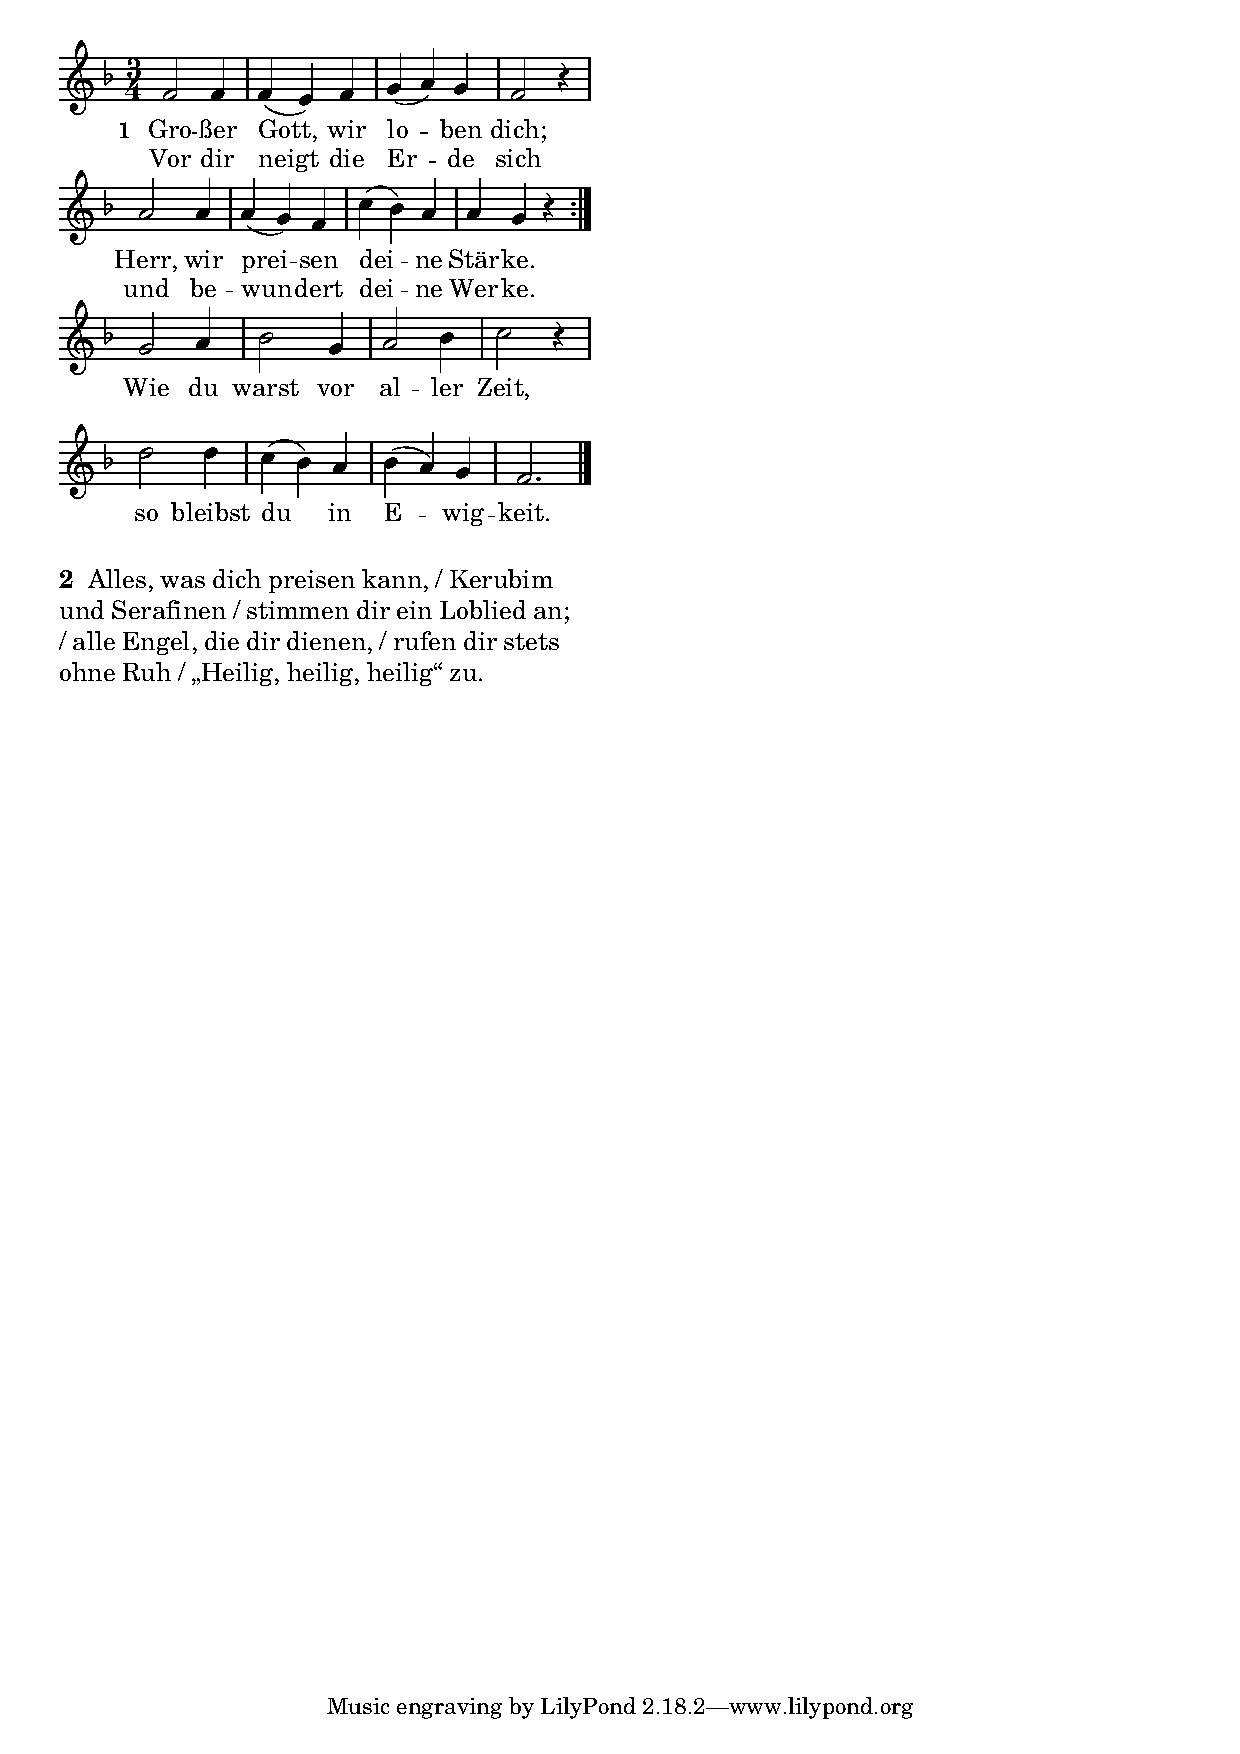
\includegraphics[width=0.64\textwidth, clip, trim=25 510 305 20]{noten/06_GrosserGott.pdf}

\vfill

\headingI{Auszug}

\headingII{Orgelspiel}
~\vfill\vspace{-1cm}
\headingII{Die Gemeinde wird gebeten die Kirche zu verlassen,\\ dann folgt das Brautpaar}
~\vfill
\footer
\end{center}

 %!TEX root=../main.tex
\setcounter{page}{1}

\begin{center}

~\vfill\vspace{-2cm}

\headingI{Einzug}

\headingII{Orgelspiel}

\vfill

\headingI{Lobe den Herren}

~\vspace{1.2em}

\headingII{GL 392, Nr. 1+4}

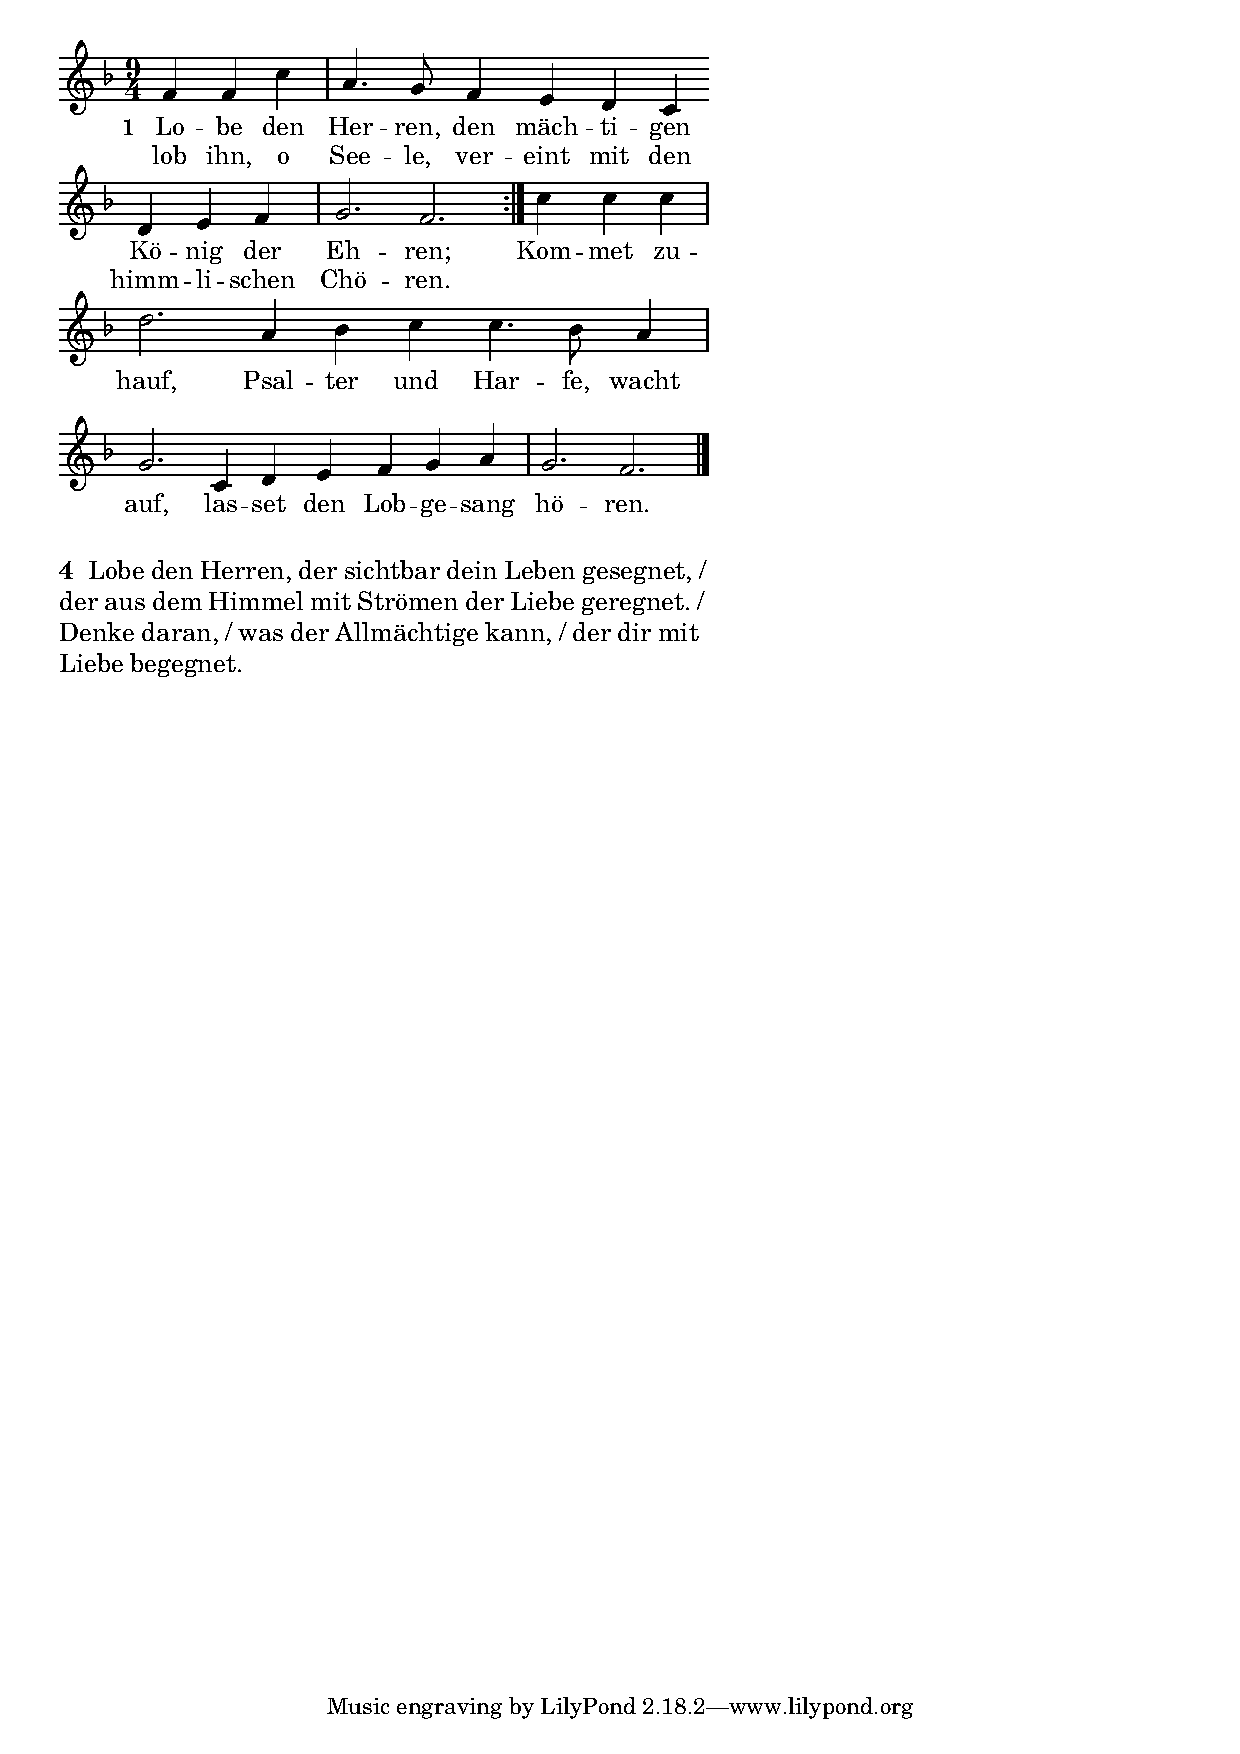
\includegraphics[width=0.75\textwidth, clip, trim=25 510 250 13]{noten/01_LobetDenHerren.pdf}

\vfill
\begruessung

\headingII{durch Pfarrer XYZ}

~\vfill

\footer
\end{center}

 %!TEX root=../main.tex
\setcounter{page}{2}

\begin{center}

~\vfill\vspace{-3cm}

\headingI{Kyrie}

\vfill

\headingI{Gloria}
~\vspace{0.6em}

\headingII{GL 172}

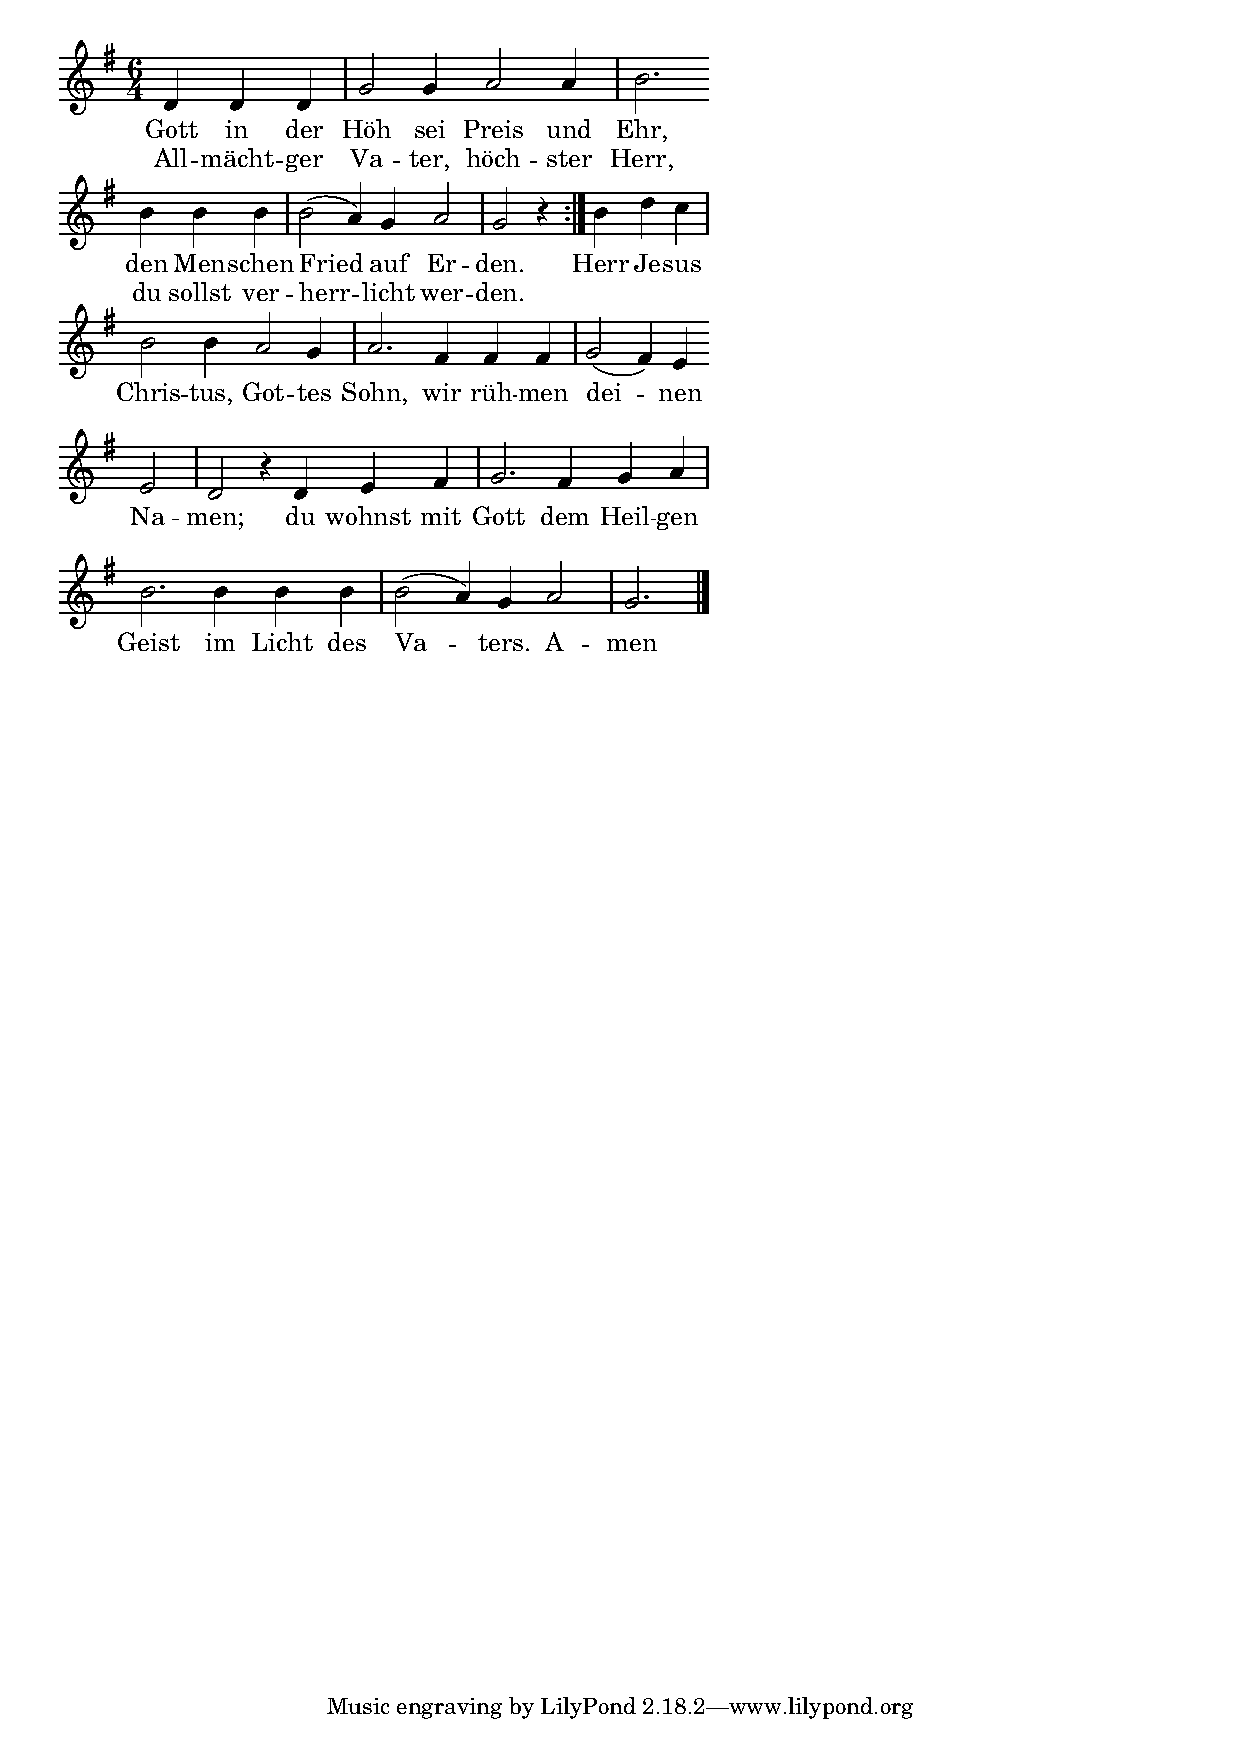
\includegraphics[width=0.75\textwidth, clip, trim=25 525 250 20]{noten/02_Gloria.pdf}

\vfill

\headingI{Tagesgebet}
\vfill

\footer

\end{center}

 %!TEX root=../main.tex
\setcounter{page}{7}
\begin{center}

~\vfill\vspace{-3cm}

\headingI{Kommunion} 
~\vspace{0.6em}

\headingII{Orgelspiel}

~\vfill

\soloI

~\vfill

\headingI{Schlusssegen}

~\vfill

\soloI

~\vfill

\footer
\end{center}

 %!TEX root=../main.tex
\setcounter{page}{6}

\begin{center}
~\vfill\vspace{-2cm}

\headingI{Sanctus} 
~\vspace{0.3em}

\headingII{GL 388}

\vspace{-0.7em}
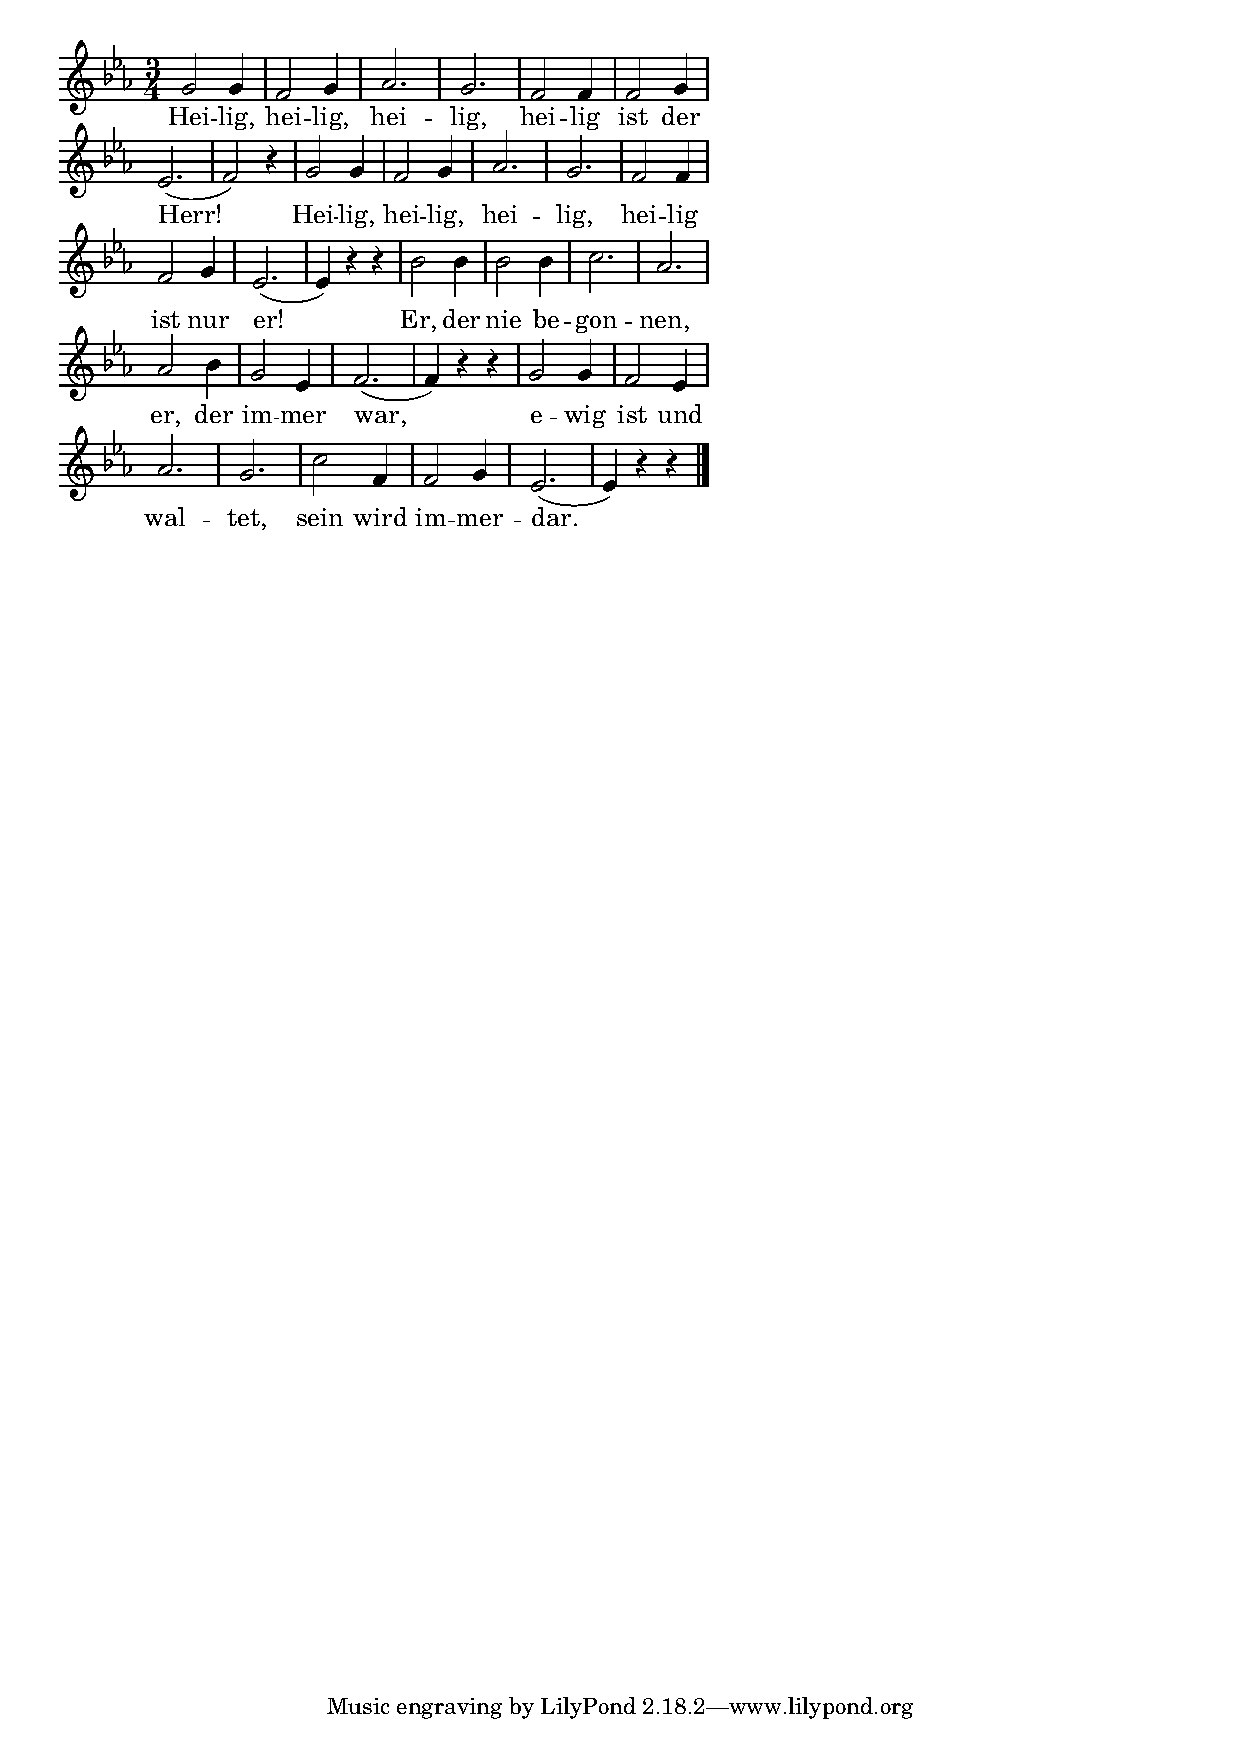
\includegraphics[width=0.75\textwidth, clip, trim=25 587 250 20]{noten/04_Sanctus.pdf}

\vfill\vspace{2em}

\headingI{Vater unser}
~\vspace{0em}

\headingII{Gesungen}

\vfill\vspace{1em}

\headingI{Agnus Dei}
~\vspace{-1.8em}

\headingII{GL 739, Nr. 1-3}

\vspace{-0.5em}
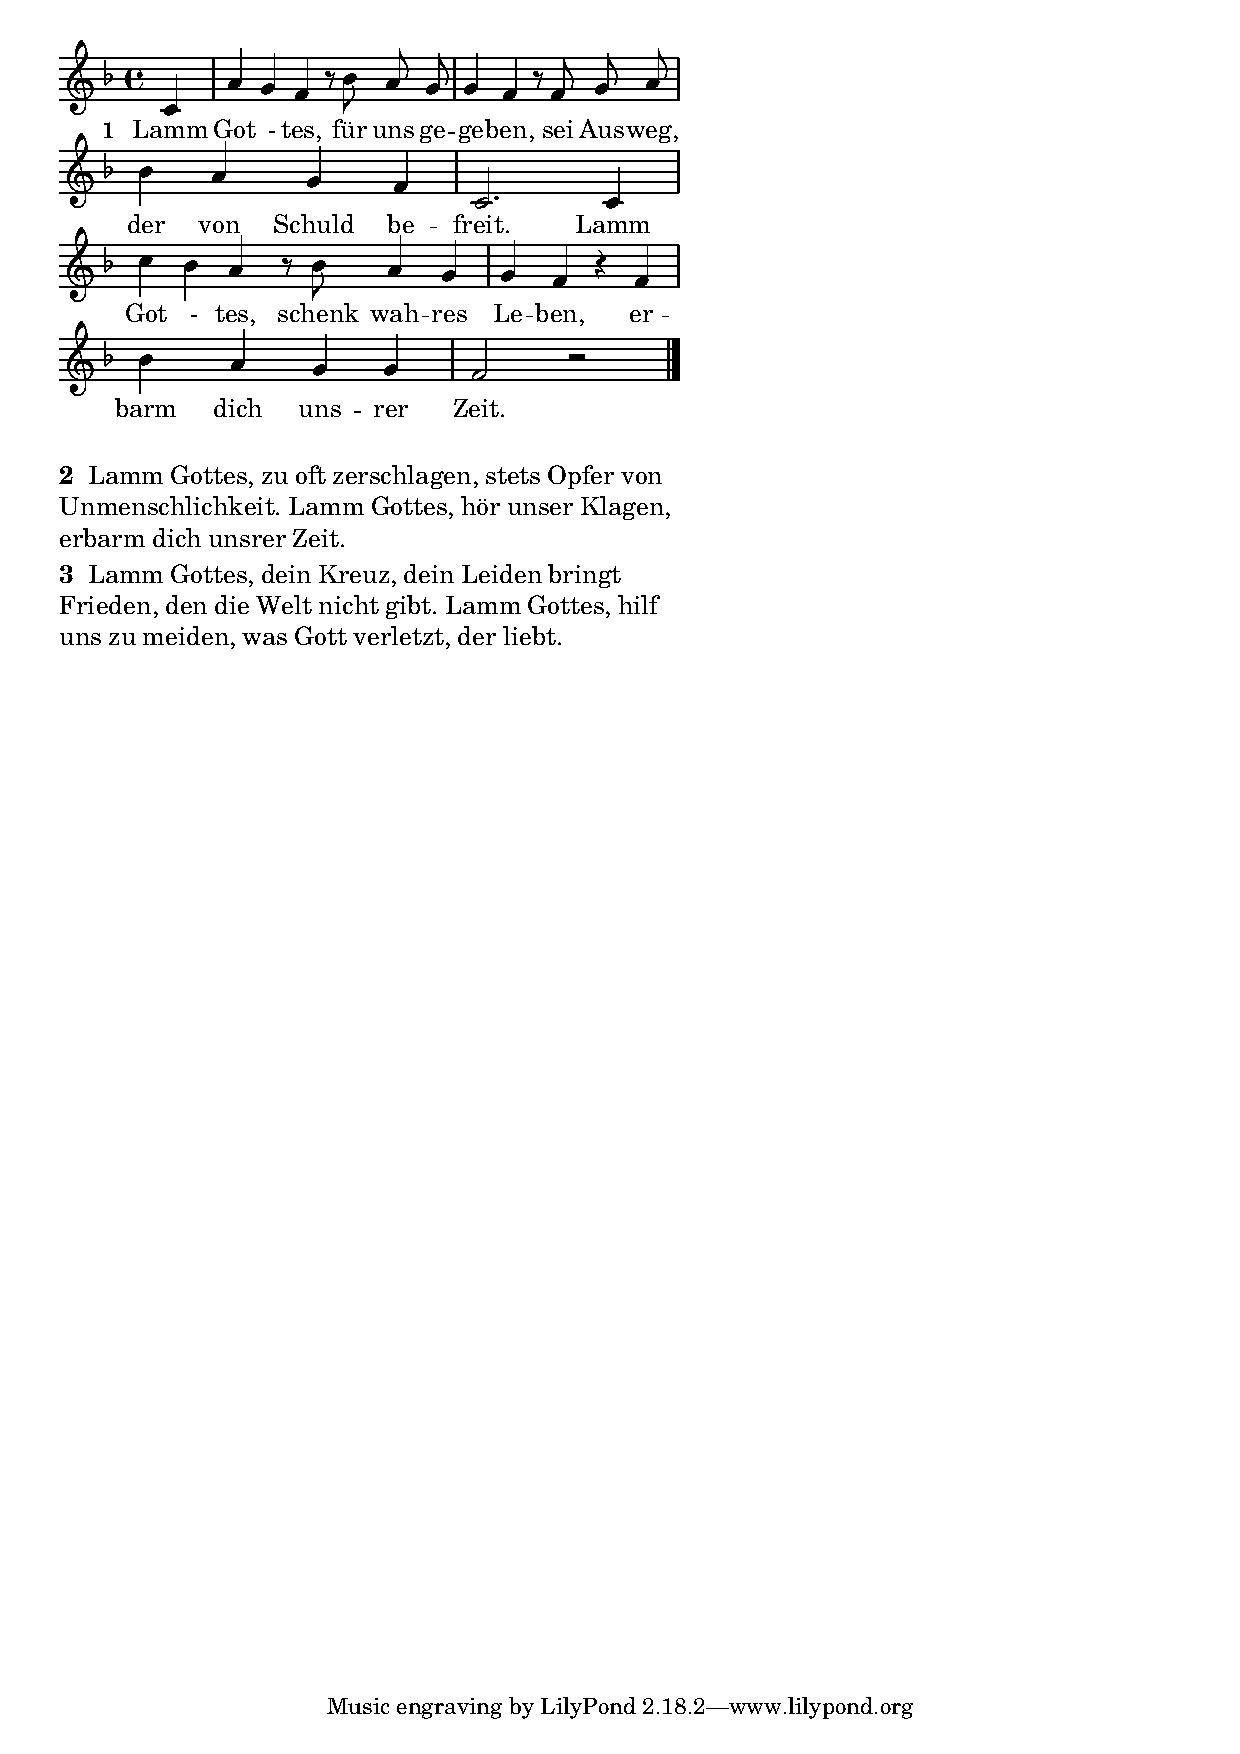
\includegraphics[width=0.75\textwidth, clip, trim=10 633 250 19]{noten/05_AgnusDei.pdf}

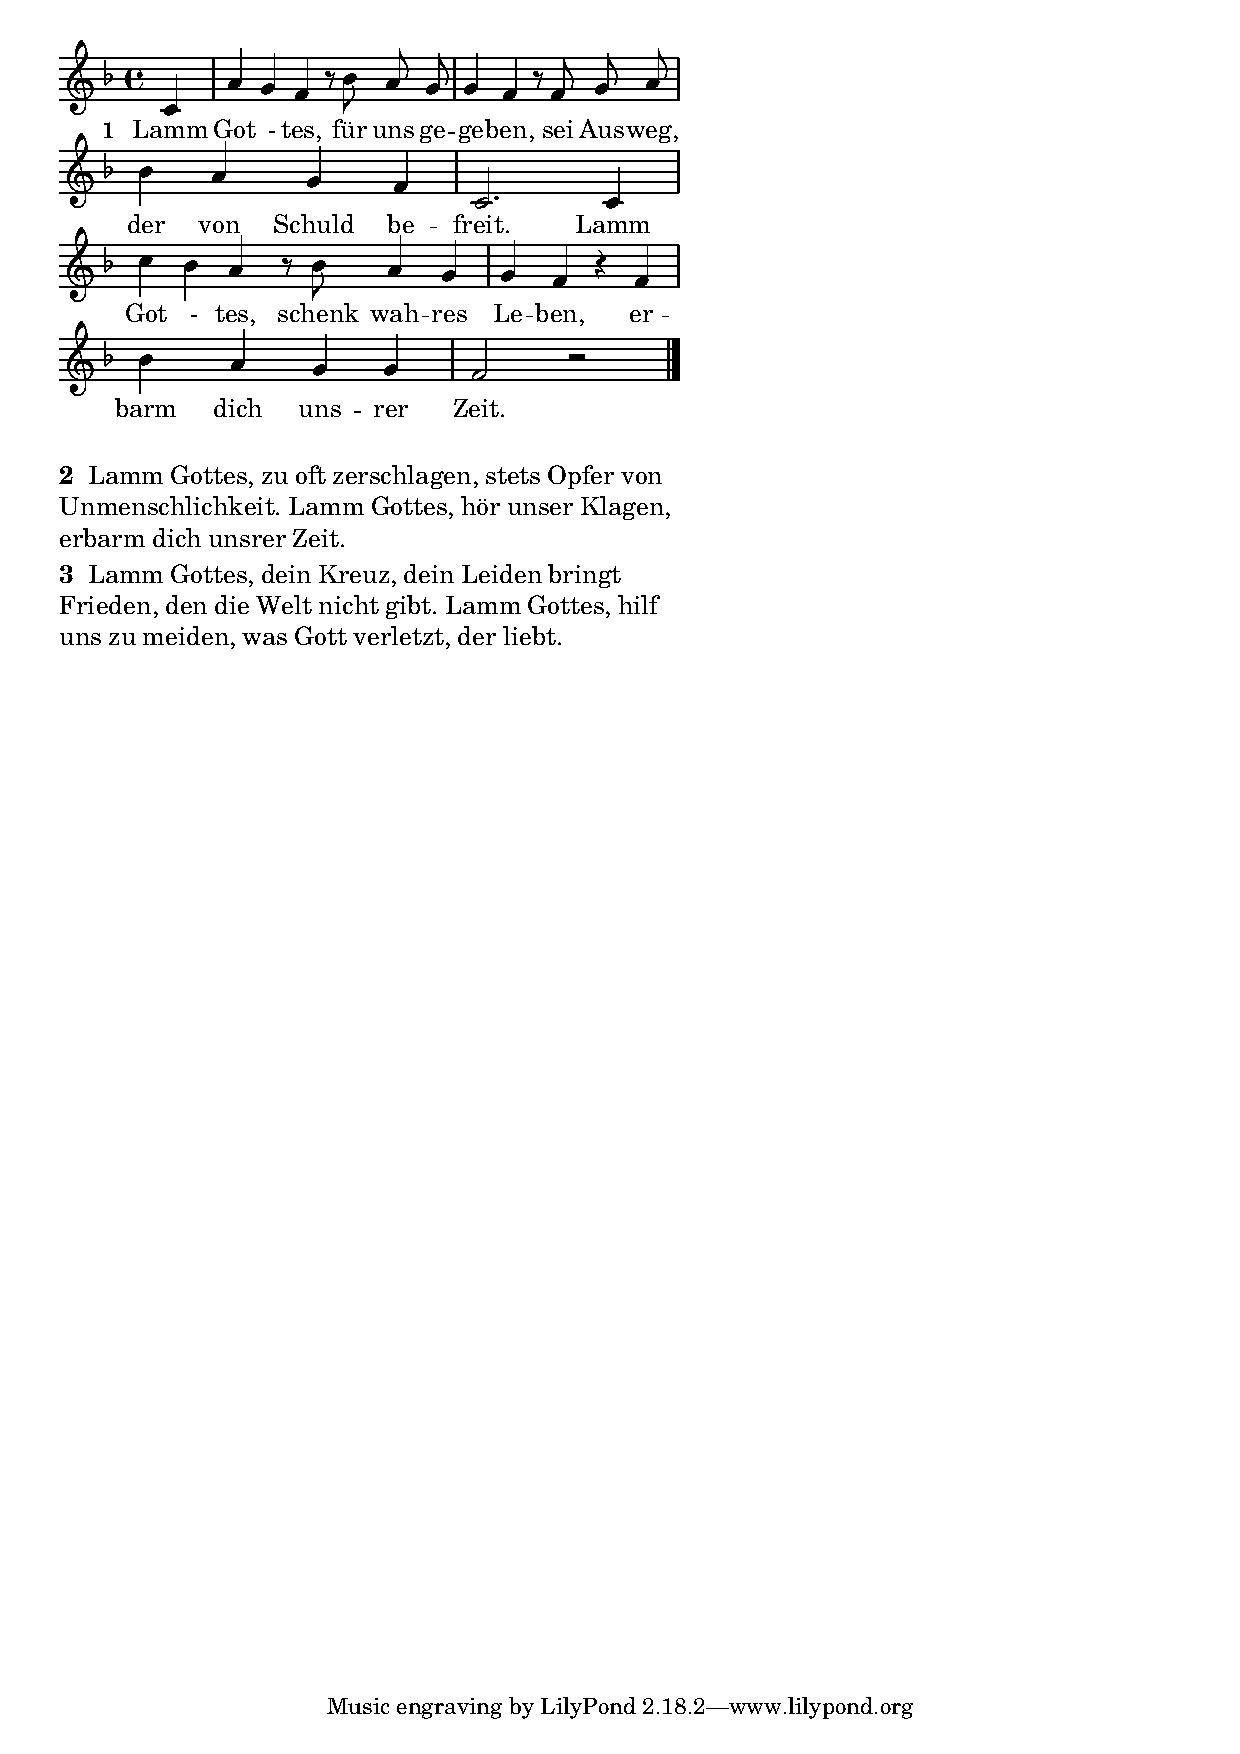
\includegraphics[width=0.75\textwidth, clip, trim=10 530 250 222]{noten/05_AgnusDei.pdf}

~\vfill\vspace{-1cm}

\footer
\end{center}

 %!TEX root=../main.tex
\setcounter{page}{3}

\begin{center}

~\vfill\vspace{-3cm}

\headingI{Lesung}

\headingII{Kol 3,12-17}

\vfill

\soloI
\vfill

\headingI{Evangelium}

~~\vspace{-1ex}

\headingII{Mk 10,6 -- 9}

~~\vspace{-2ex}

\headingII{\glqq Sie sind nicht mehr zwei,}
\vspace{-1ex}

\headingII{sondern eins\grqq}

\vfill


\headingI{Predigt}

~\vfill

\footer

\end{center}

 %!TEX root=../main.tex

\setcounter{page}{5}

\begin{center}

~\vfill\vspace{-3cm}

\headingI{Trauung}
\vfill
\headingI{Eheversprechen}
\vfill
\headingI{Trausegen}
\vfill
\soloI

\vfill
\footer

\end{center}

 %!TEX root=../main.tex
\setcounter{page}{5}

\begin{center}

\headingI{Fürbitten}

\vfill

\headingI{Gabenbereitung}
~\vspace{-0.8em}

\headingII{GL 470, Nr. 1+3}

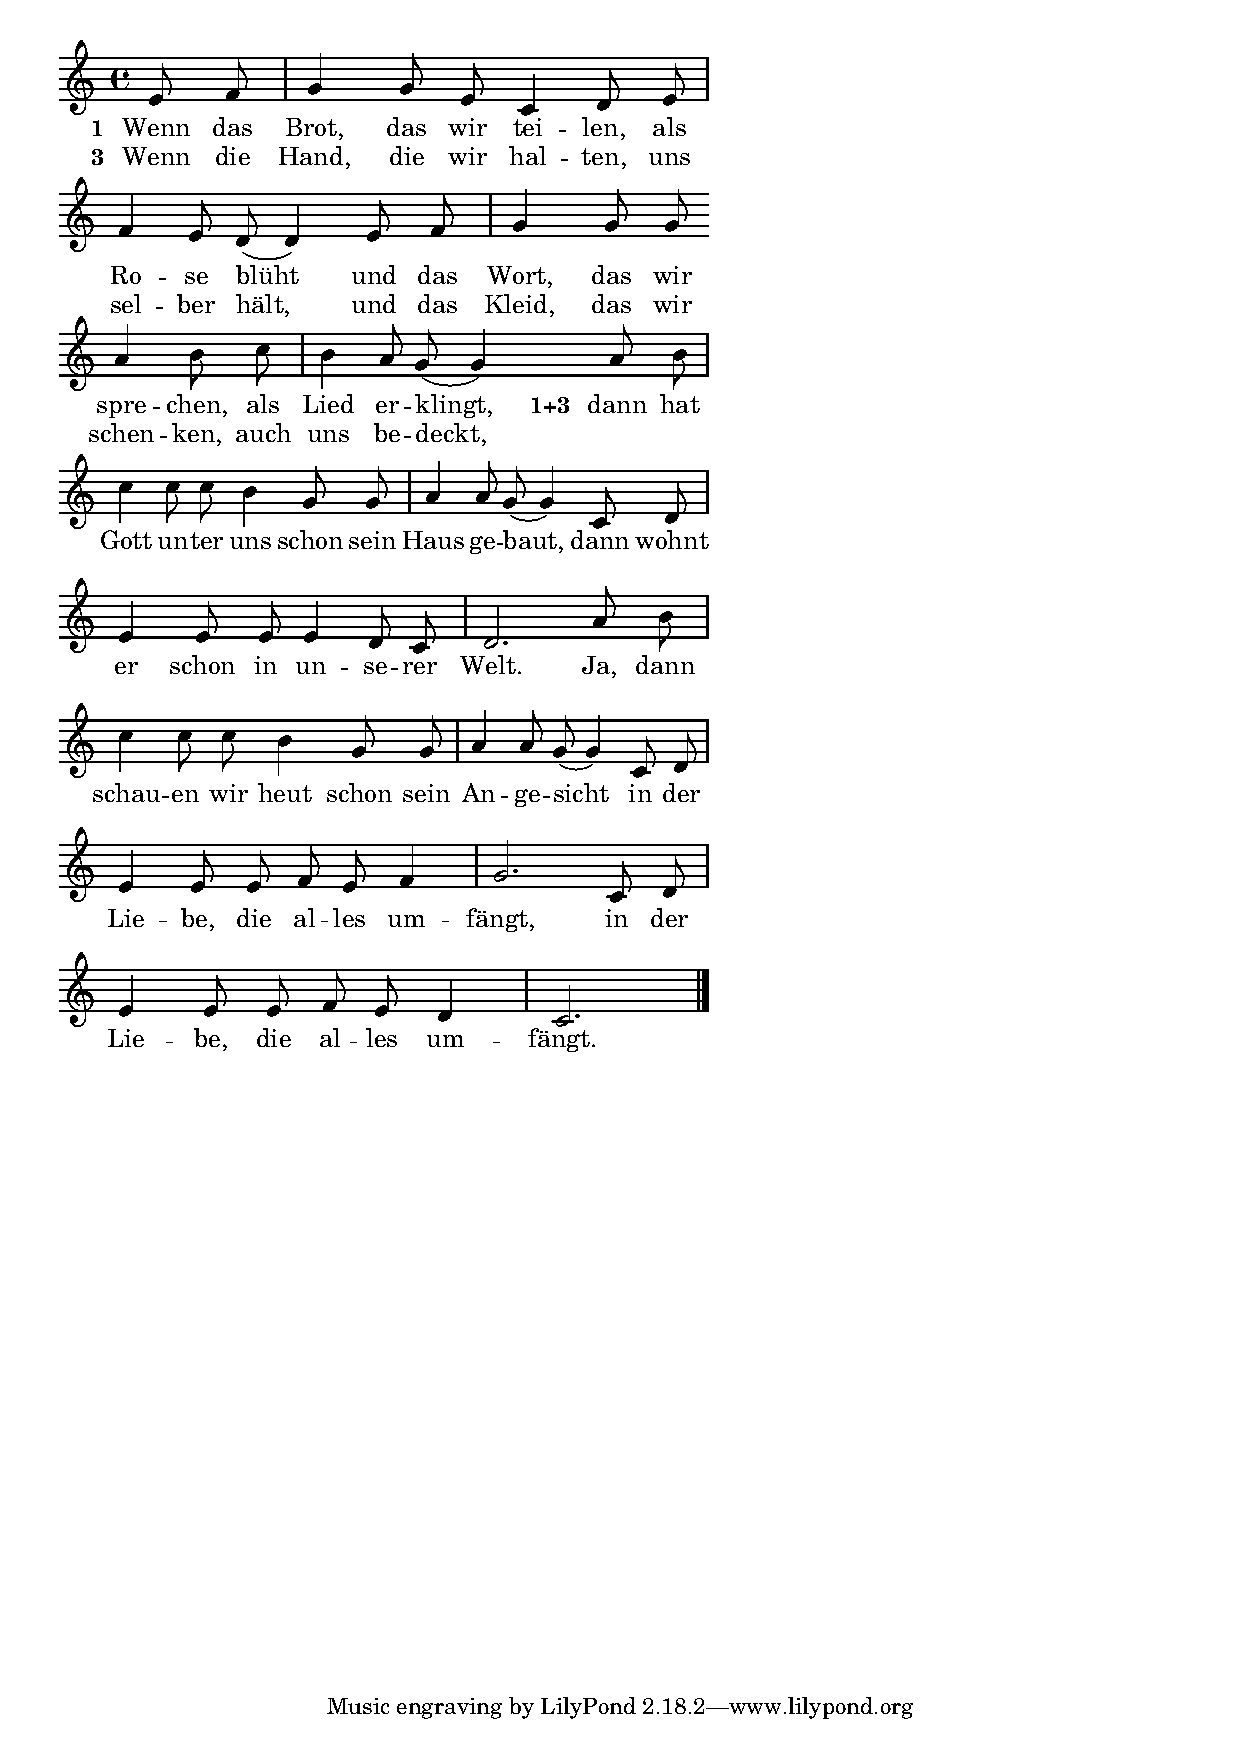
\includegraphics[width=0.75\textwidth, clip, trim=25 330 240 15]{noten/03_Gabenbereitung.pdf}
\vfill


\footer

\end{center}

}
{
%%%%%%%%%%%%%%%%%%%%%%%%%%%%%%%%%%%%%%%
%		Reihenfolge zur Ansicht	      %
%%%%%%%%%%%%%%%%%%%%%%%%%%%%%%%%%%%%%%%

\gI

%!TEX root=../main.tex
\thispagestyle{empty}

\begin{center}

~\vfill\vspace{-1.5cm}
\headingCIII{Kirchliche Trauung}

\vspace{2ex}

\headingCI{\huge\calligra{\hspace{-0ex}{Name\hspace{-0ex} \& \hspace{-1.2ex}Name}}}

~\vfill\vspace{-0.5cm}

\begin{tikzpicture}{remember picture, overlay}
\clip (3.9,-5.7) circle (0.44\textwidth);
\end{tikzpicture}

~\vfill\vspace{-0.5cm}

\headingCIV{Datum}\\
\headingCIV{Pfarrei}\\
\headingCIV{Ort}\\

\end{center}

\restoregeometry

%!TEX root=../main.tex

\thispagestyle{empty}
\begin{center}

\headingCIV{
\glqq Wichtiger als alles andere ist die Liebe.\\[0.2em] Wenn ihr sie habt, wird euch nichts fehlen.\\[0.2em] Sie ist das Band, das euch verbindet.\grqq
}
~\vspace{-2ex}
\end{center}

\begin{center}
\fmmfamily\textit{Kol 3,14}

\vfill

\end{center}



\clearpage

\gII

%!TEX root=../main.tex
\setcounter{page}{1}

\begin{center}

~\vfill\vspace{-2cm}

\headingI{Einzug}

\headingII{Orgelspiel}

\vfill

\headingI{Lobe den Herren}

~\vspace{1.2em}

\headingII{GL 392, Nr. 1+4}

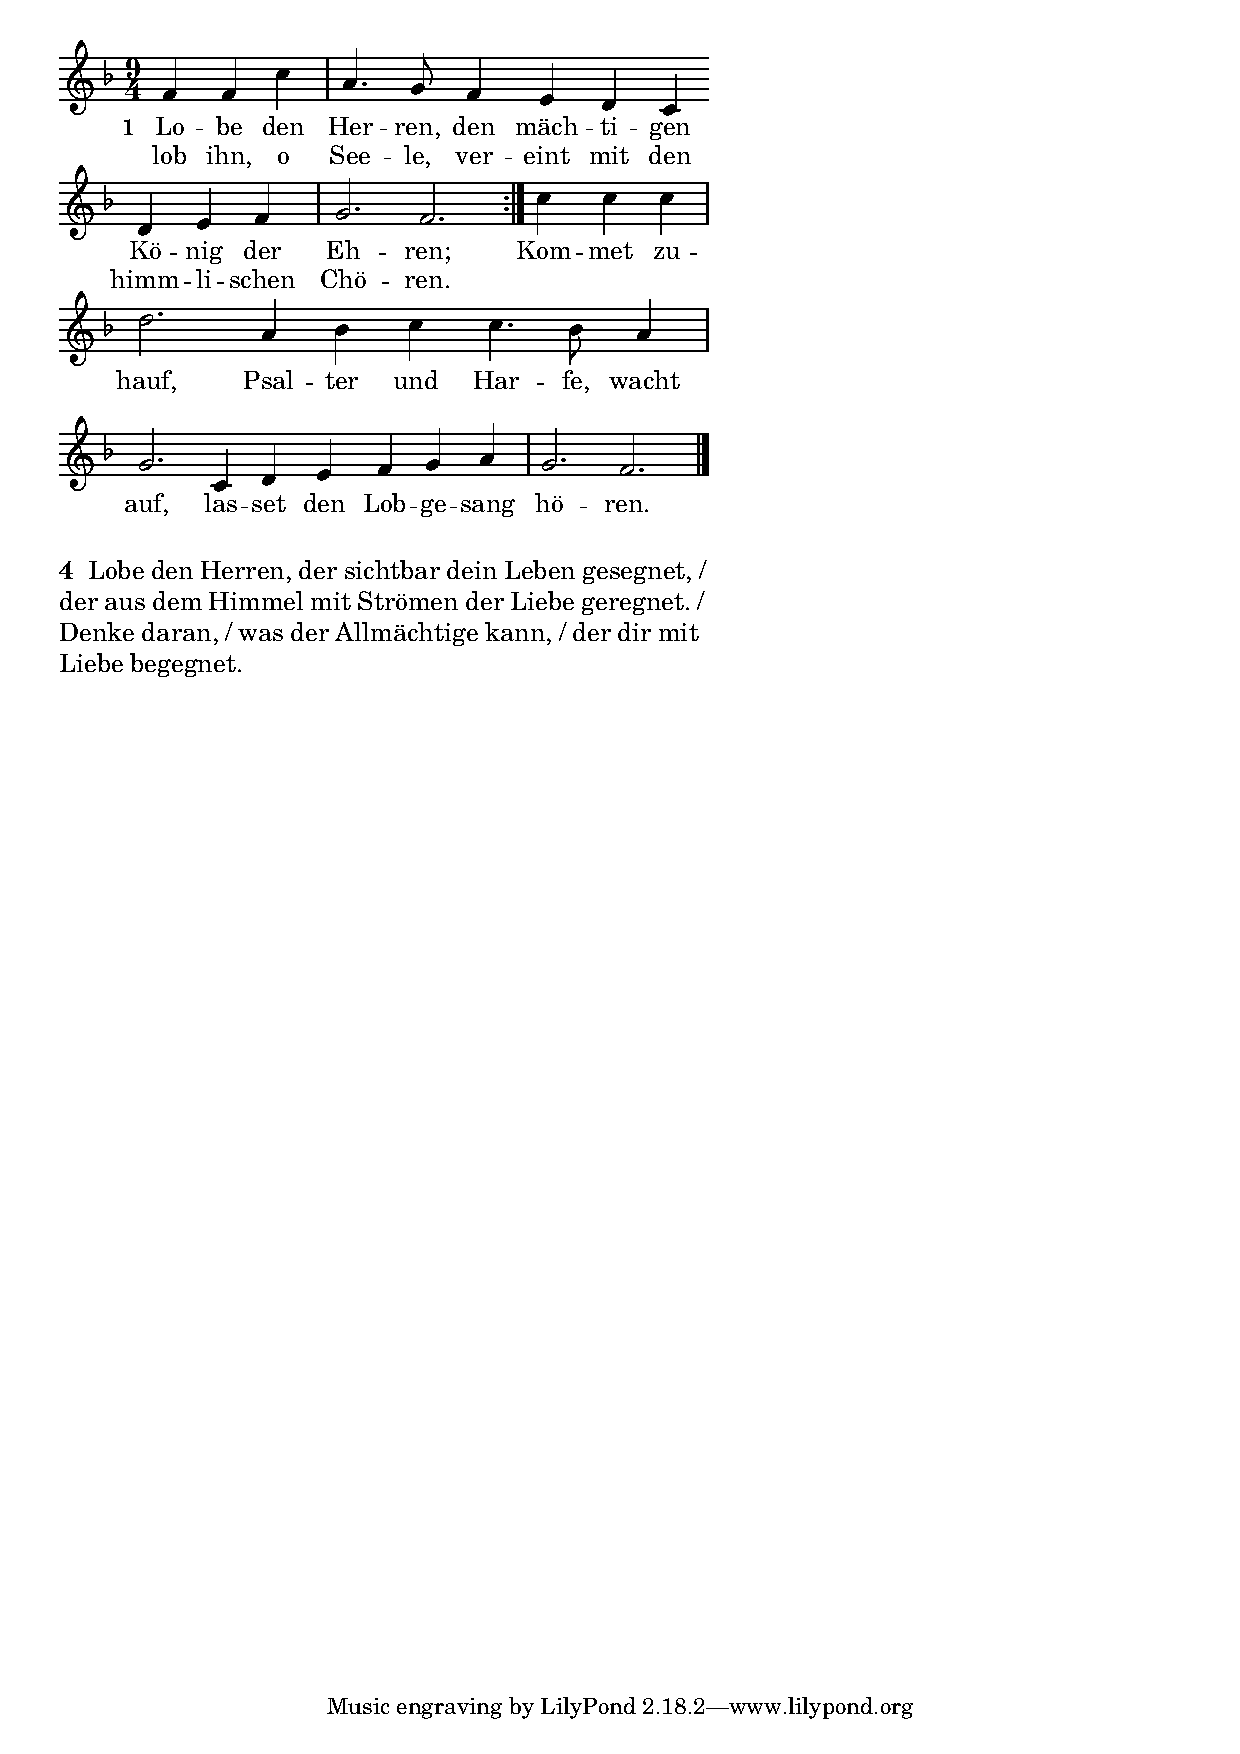
\includegraphics[width=0.75\textwidth, clip, trim=25 510 250 13]{noten/01_LobetDenHerren.pdf}

\vfill
\begruessung

\headingII{durch Pfarrer XYZ}

~\vfill

\footer
\end{center}

%!TEX root=../main.tex
\setcounter{page}{2}

\begin{center}

~\vfill\vspace{-3cm}

\headingI{Kyrie}

\vfill

\headingI{Gloria}
~\vspace{0.6em}

\headingII{GL 172}

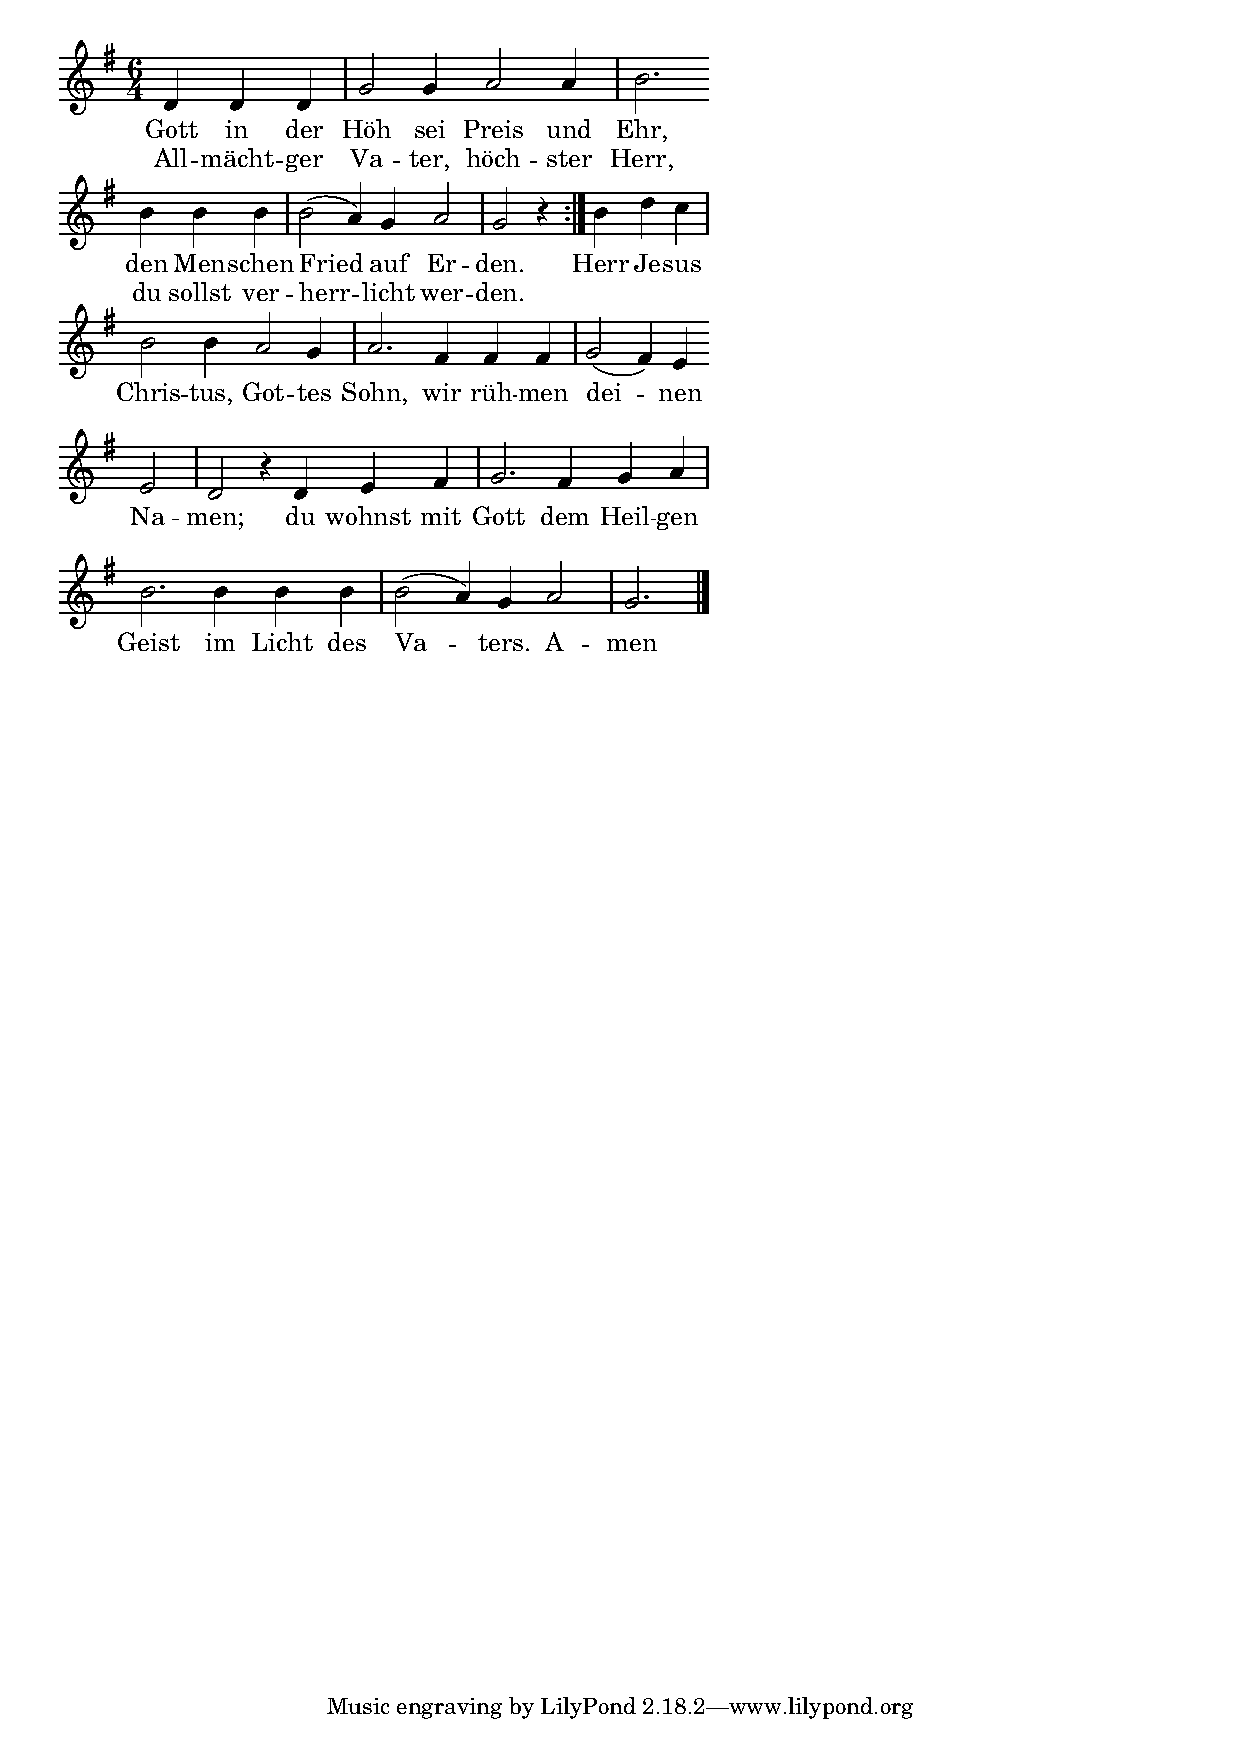
\includegraphics[width=0.75\textwidth, clip, trim=25 525 250 20]{noten/02_Gloria.pdf}

\vfill

\headingI{Tagesgebet}
\vfill

\footer

\end{center}

%!TEX root=../main.tex
\setcounter{page}{3}

\begin{center}

~\vfill\vspace{-3cm}

\headingI{Lesung}

\headingII{Kol 3,12-17}

\vfill

\soloI
\vfill

\headingI{Evangelium}

~~\vspace{-1ex}

\headingII{Mk 10,6 -- 9}

~~\vspace{-2ex}

\headingII{\glqq Sie sind nicht mehr zwei,}
\vspace{-1ex}

\headingII{sondern eins\grqq}

\vfill


\headingI{Predigt}

~\vfill

\footer

\end{center}

%!TEX root=../main.tex

\setcounter{page}{5}

\begin{center}

~\vfill\vspace{-3cm}

\headingI{Trauung}
\vfill
\headingI{Eheversprechen}
\vfill
\headingI{Trausegen}
\vfill
\soloI

\vfill
\footer

\end{center}

%!TEX root=../main.tex
\setcounter{page}{5}

\begin{center}

\headingI{Fürbitten}

\vfill

\headingI{Gabenbereitung}
~\vspace{-0.8em}

\headingII{GL 470, Nr. 1+3}

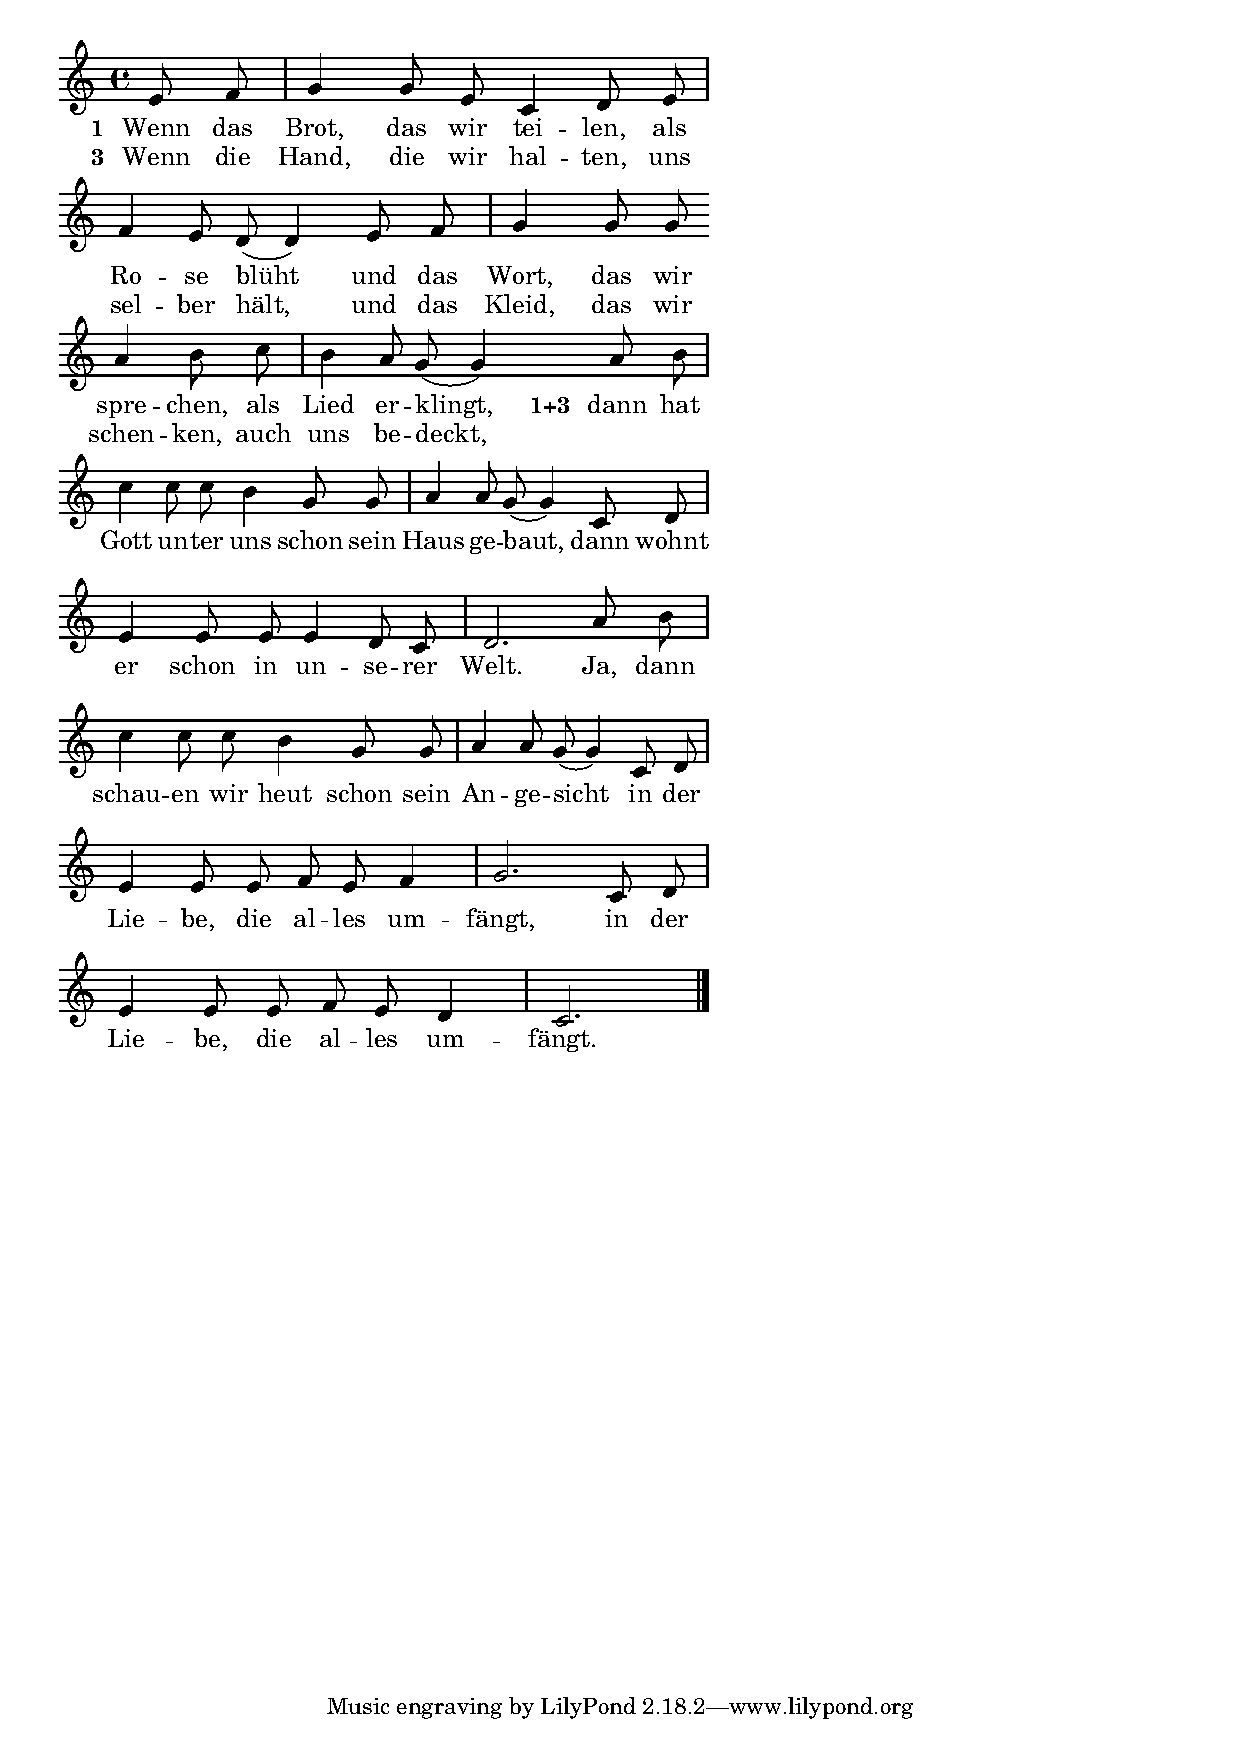
\includegraphics[width=0.75\textwidth, clip, trim=25 330 240 15]{noten/03_Gabenbereitung.pdf}
\vfill


\footer

\end{center}

%!TEX root=../main.tex
\setcounter{page}{6}

\begin{center}
~\vfill\vspace{-2cm}

\headingI{Sanctus} 
~\vspace{0.3em}

\headingII{GL 388}

\vspace{-0.7em}
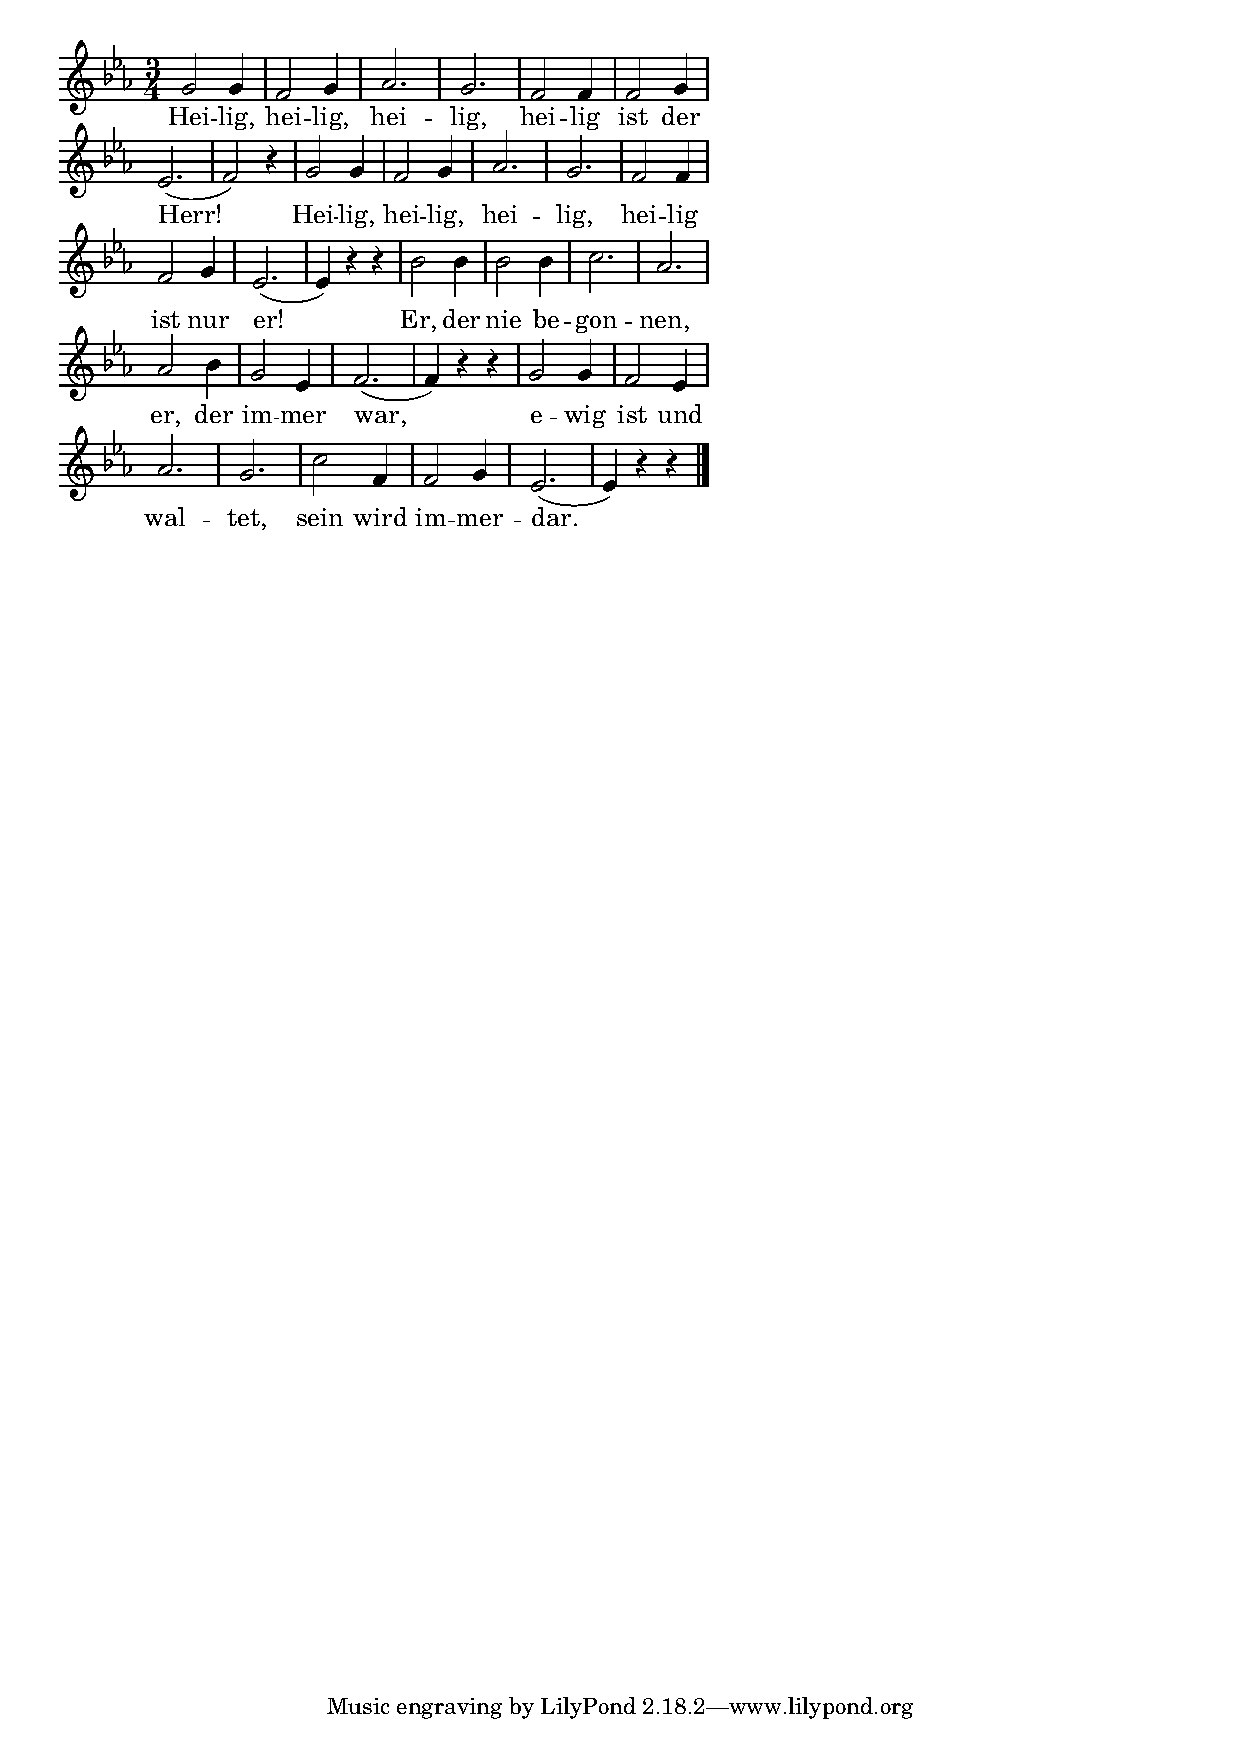
\includegraphics[width=0.75\textwidth, clip, trim=25 587 250 20]{noten/04_Sanctus.pdf}

\vfill\vspace{2em}

\headingI{Vater unser}
~\vspace{0em}

\headingII{Gesungen}

\vfill\vspace{1em}

\headingI{Agnus Dei}
~\vspace{-1.8em}

\headingII{GL 739, Nr. 1-3}

\vspace{-0.5em}
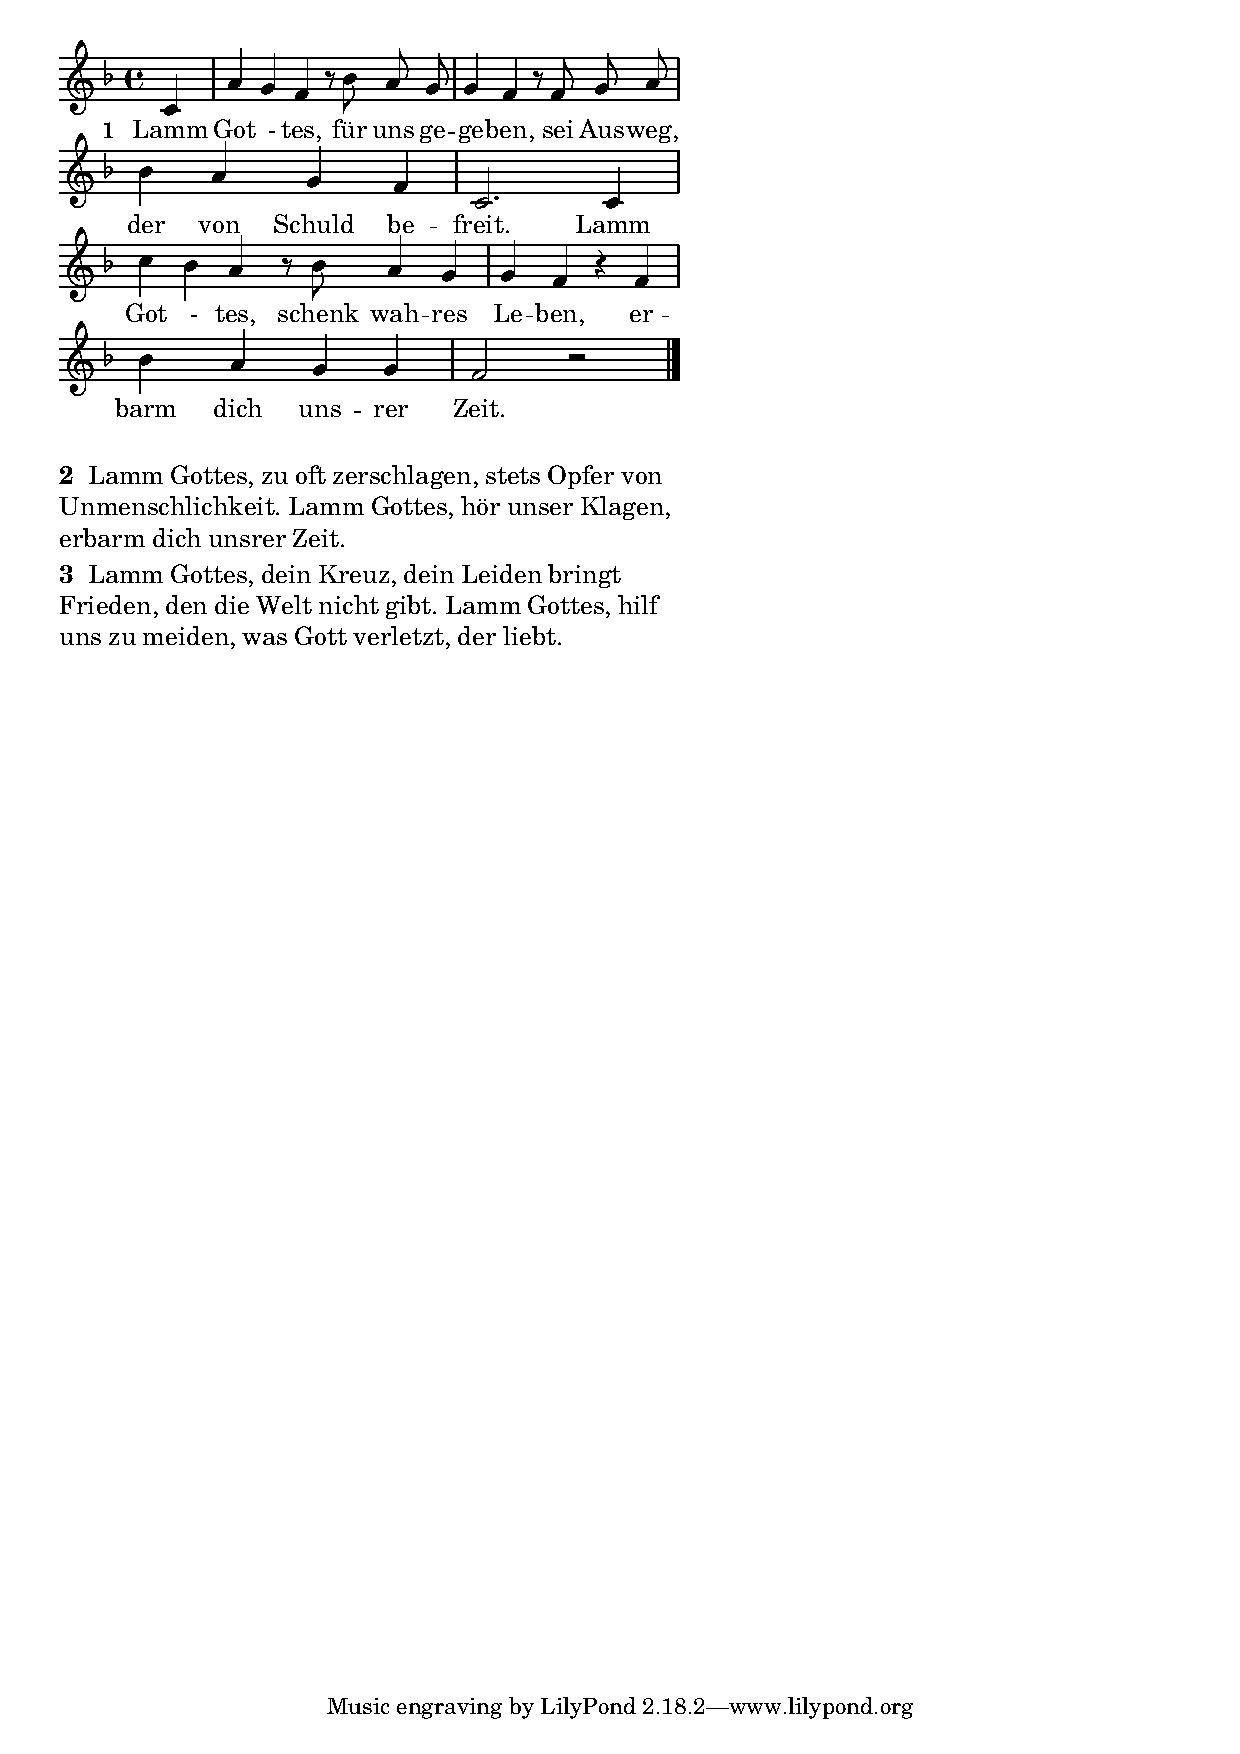
\includegraphics[width=0.75\textwidth, clip, trim=10 633 250 19]{noten/05_AgnusDei.pdf}

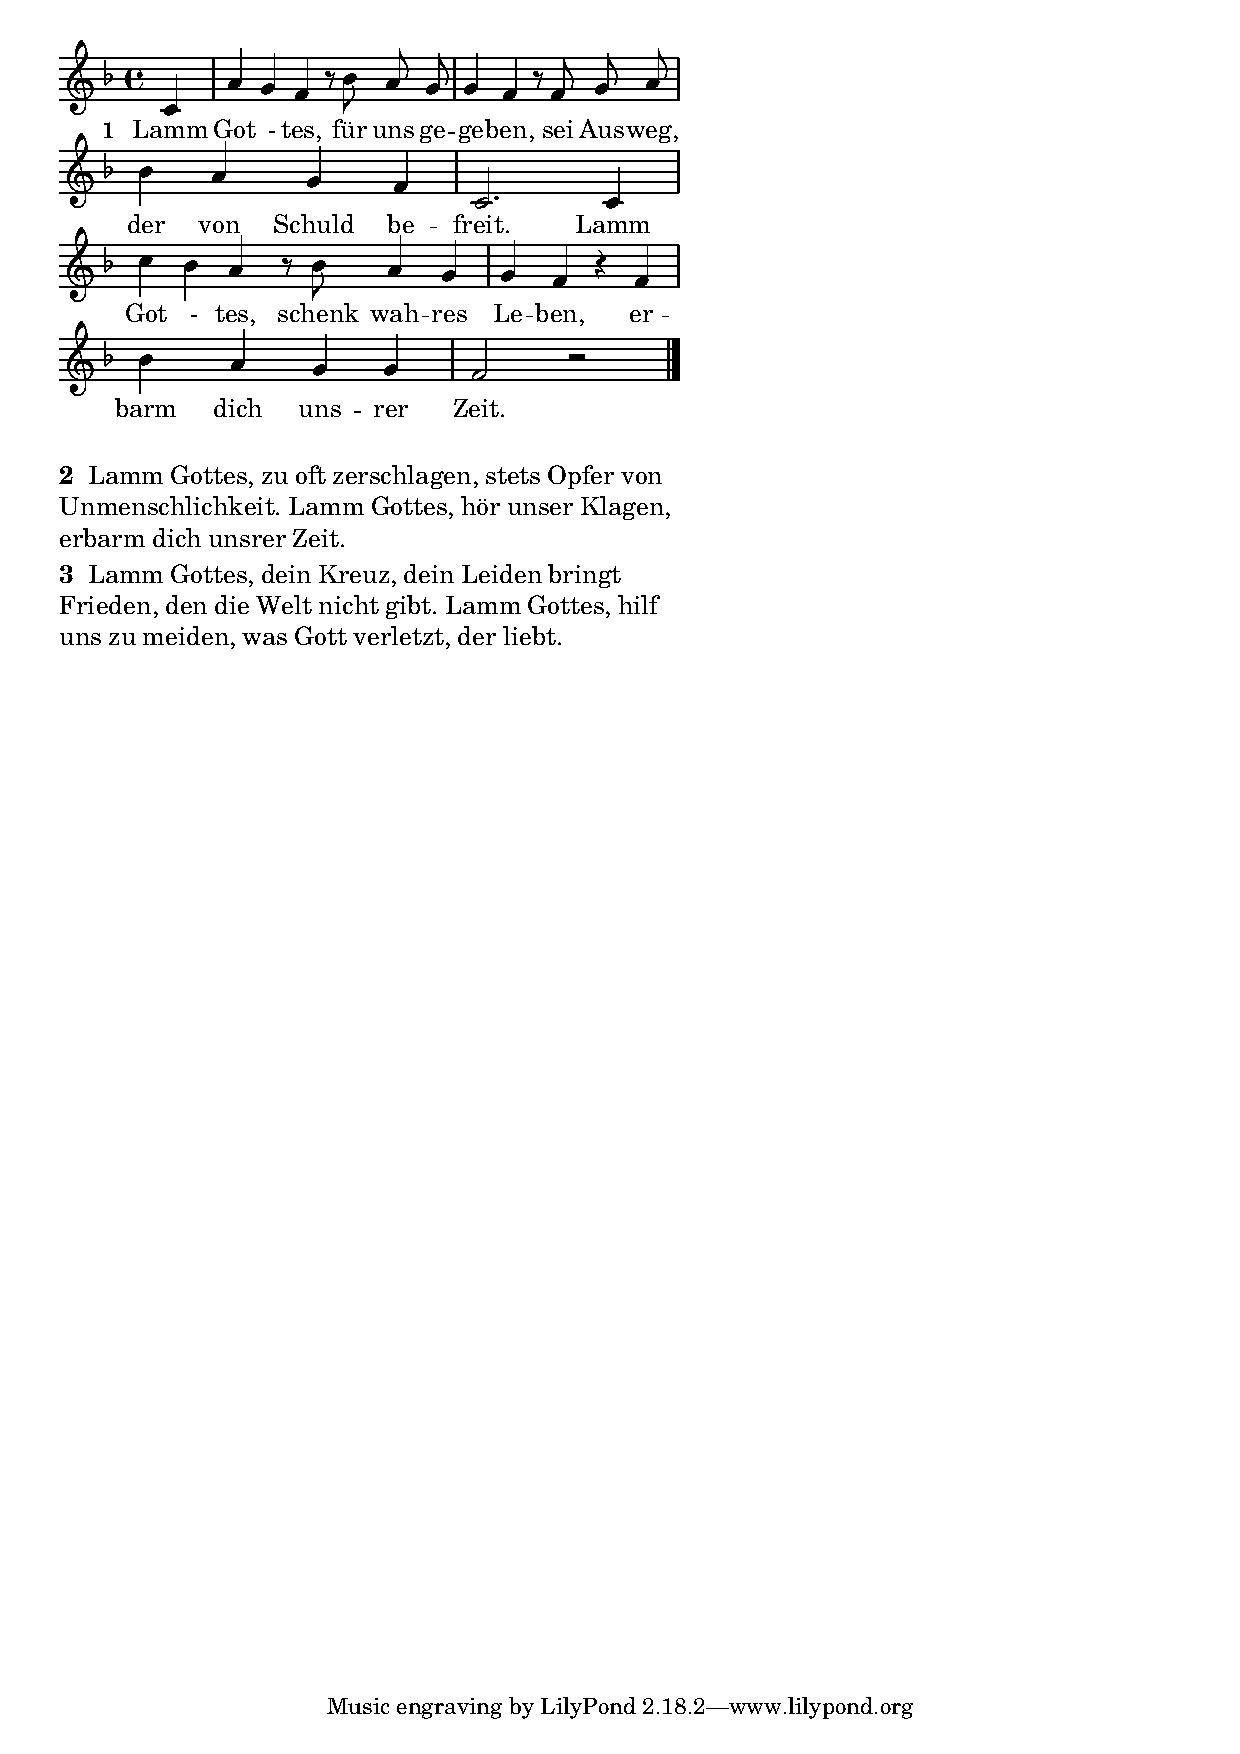
\includegraphics[width=0.75\textwidth, clip, trim=10 530 250 222]{noten/05_AgnusDei.pdf}

~\vfill\vspace{-1cm}

\footer
\end{center}

%!TEX root=../main.tex
\setcounter{page}{7}
\begin{center}

~\vfill\vspace{-3cm}

\headingI{Kommunion} 
~\vspace{0.6em}

\headingII{Orgelspiel}

~\vfill

\soloI

~\vfill

\headingI{Schlusssegen}

~\vfill

\soloI

~\vfill

\footer
\end{center}

%!TEX root=../main.tex
\setcounter{page}{8}
\begin{center}

~\vfill\vspace{-2cm}

\headingI{Großer Gott, wir loben dich}
~\vspace{-0.4em}

\headingII{GL 380, Nr. 1+2}

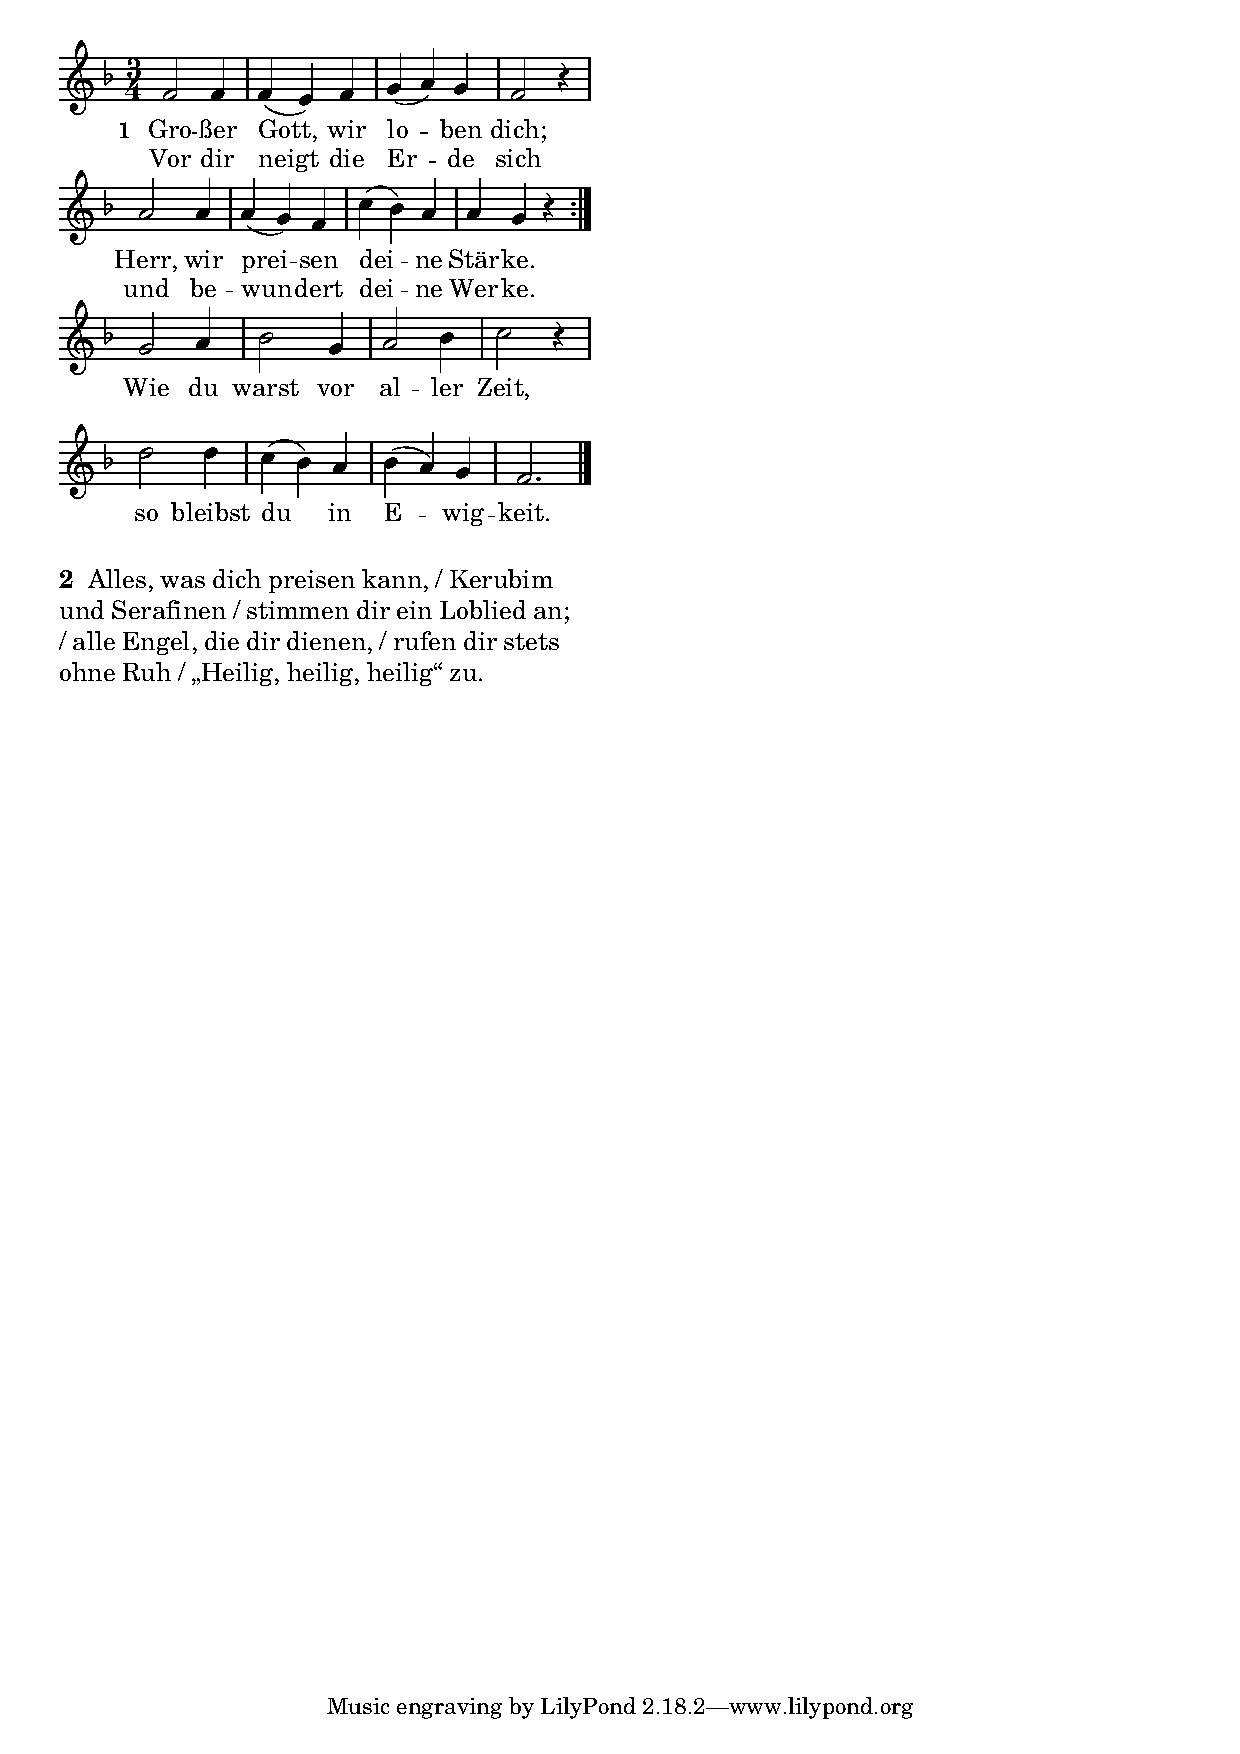
\includegraphics[width=0.64\textwidth, clip, trim=25 510 305 20]{noten/06_GrosserGott.pdf}

\vfill

\headingI{Auszug}

\headingII{Orgelspiel}
~\vfill\vspace{-1cm}
\headingII{Die Gemeinde wird gebeten die Kirche zu verlassen,\\ dann folgt das Brautpaar}
~\vfill
\footer
\end{center}

%!TEX root=../main.tex
\thispagestyle{empty}

\begin{center}

\begin{tikzpicture}{remember picture, overlay}
\put(-70,-600){

\includegraphics[width=0.28\textwidth]{img/herzBlume.pdf};}
\end{tikzpicture}

\headingCII{Danke}\vspace{2ex}
\headingCIII{
\begin{flushleft}
\begin{tabularx}{\textwidth}{lZ}
\tableI \textbf\dots & \tableI sagen wir allen, die heute zu unserer Hochzeit gekommen sind und diesen Gottesdienst mit uns gefeiert und mitgestaltet haben.\\[0.2em]
\tableI \textbf\dots & \tableI sagen wir besonders unseren Eltern, Familie, Trauzeugen und Freunden, die uns auf unserem bisherigen Lebensweg begleitet und unterstützt haben.\\[0.2em]
\tableI \textbf\dots & \tableI sagen wir Pfarrer XYZ für die persönliche Gestaltung unserer Trauung.\\[0.2em]
\tableI \textbf\dots & \tableI sagen wir allen, die uns bei der Gestaltung und Organisation unserer Hochzeit geholfen haben.\\[0.2em]
\tableI \textbf\dots & \tableI euch allen, dass ihr diesen Tag zu einem ganz besonderen macht.\\[0em]
\end{tabularx}
\end{flushleft}
}

\vfill

\end{center}
}




\end{document}